\chapter{Teil 2: Klassifikation}
\section{Einleitung}\label{sec:classification}
Um eine Klassifizierung durchführen zu können, sind mehrere Komponenten notwendig, welche miteinander arbeiten. 
Dieser Ablauf wird in der \cref{fig:ablauf_klassifizierung} gezeigt.
\begin{figure}[H]	
	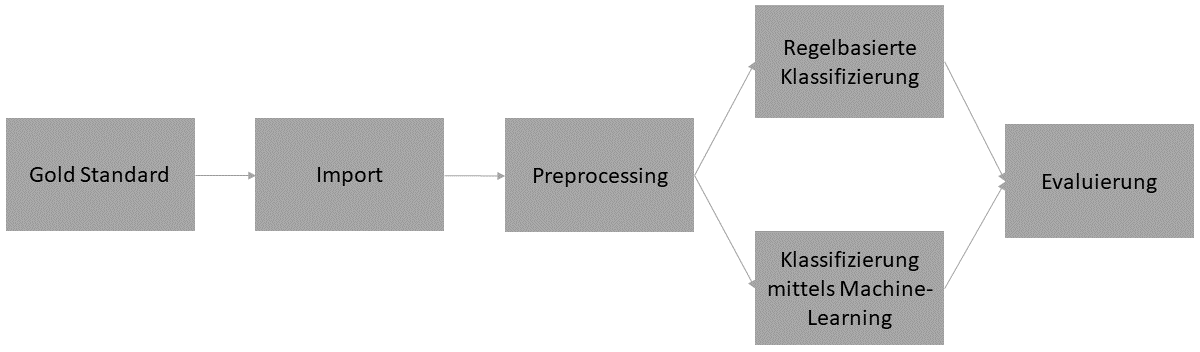
\includegraphics[width=1\columnwidth,keepaspectratio]{img/Ablauf_Klassifizierung.png}
	\caption{Pipeline}
	\label{fig:ablauf_klassifizierung}
\end{figure}
Als Grundlage dienen die Daten des Gold Standards.
Diese werden mittels einer Import-Komponente geladen.
Bevor die Daten mit den entsprechenden Methoden klassifiziert werden, werden sie bei Bedarf noch vorverarbeitet.
Dann findet die eigentliche Klassifizierung statt.
Um eine möglichst präzise und erfolgreiche Variante des Klassifizierens zu finden, werden in diesem Teil der Arbeit mehrere Experimente durchgeführt.
Zum Schluss folgt eine Komponente, welche für das Auswerten der Klassifizierung und Ausgeben der Ergebnisse verantwortlich ist.
\section{Preprocessing}
Das Preprocessing wurde entwickelt, um den Inhalt des Dokuments auf eine standardisierte Form zu bringen.
Die folgenden Methoden können sowohl auf den Text eines Dokuments sowie auch auf den Titel angewendet werden.
Sie können mittels Konfiguration sowohl für den Text als auch Titel eines Dokuments ein- oder ausgeschaltet werden.
\subsection{Basis Preprocessing}
Um Text besser klassifizieren zu können, muss dieser zuerst bereinigt und standardisiert werden\footnote{\url{https://machinelearningmastery.com/clean-text-machine-learning-python/} abgerufen am: 11.07.2019}.
Die nachfolgenden Methoden des Basis Preprocessing werden in jedem Fall der Klassifikation durchgeführt.
Sie verändern jeweils nur einzelne Zeichen des Textes.
\subsubsection{Gross-/Kleinschreibung}
Alle Buchstaben, welche grossgeschrieben sind, werden durch die entsprechenden Kleinbuchstaben ersetzt.
\subsubsection{Umlaute ersetzen}
Umlaute werden durch ihre verwandten Selbstlaute ersetzt, genauer:
\begin{itemize}
	\item ä $\rightarrow$ a
	\item ö $\rightarrow$ o
	\item ü $\rightarrow$ u
\end{itemize} 
\subsubsection{Sonderzeichen entfernen}
Alle Sonderzeichen, die nicht in der folgenden Auflistung vorkommen, werden durch einen Leerschlag ersetzt:
\begin{itemize}
	\item éàèÉÀÈäöüÄÖÜa-zA-Z
\end{itemize} 
\subsubsection{Einzelne Zeichen entfernen}
Jedes einzelne Zeichen, also solche, die sowohl vorne als auch hinten an einen Leerschlag angrenzen, werden entfernt.
\subsubsection{Multiple Leerschläge entfernen}
Da durch die vorhergehenden Schritte oft multiple Leerschläge anfallen, werden diese auf einen Leerschlag reduziert.
\subsection{Erweiterte Preprocessing}
Die nachfolgenden Methoden stellen das erweiterte Preprocessing dar.
Im Gegensatz zum Basis Preprocessing ersetzen, löschen oder verändern sie ganze Wörter im Text.
\subsubsection{Preisdetektor}
Da Menüs häufig in Verbindung mit Preisen vorkommen und in weiteren Preprocessing-Schritten Zahlen und Sonderzeichen entfernt werden, ist es von Vorteil, diese Informationen nicht zu verlieren.
Daher erkennt diese Methode verschiedene Varianten von Preisen mittels Regulären Ausdrücken (Regex, Regular Expression) und ersetzt diese mit einem Schlüsselwort.
% Varianten genauer ausführen
Die folgenden Varianten von Preisen wird erkannt:
\begin{itemize}
	\item Preisangabe + chf/fr/sfr
	\item Preisangabe
	\item chf/fr/sfr + Preisangabe
\end{itemize} 
Zudem wird unterschieden, wie viele Stellen der Preis hat.
Die nun aufgeführte Liste zeigt die verschiedenen Schlüsselwörter:
\begin{itemize}
	\item Einstellig $\rightarrow$ onedigitprice
	\item Zweistellig $\rightarrow$ twodigitprice
	\item Dreistellig $\rightarrow$ threedigitprice
\end{itemize} 
Um Zeitangaben nicht als Preise zu erkennen, werden bei Preisangaben ohne Währungsangabe nur Beträge mit Rappenbeträgen, welche 60 oder höher sind, erkannt.
\subsubsection{Stammformreduktion}
Dieses Verfahren führt verschiedene morphologische Varianten eines Wortes auf ihren gemeinsamen Stamm zurück.
Dafür wird der Stemmer \glqq Cistem\footnote{\url{https://github.com/LeonieWeissweiler/CISTEM} abgerufen am: 18.03.2019}\grqq{} verwendet, da für die deutsche Sprache nur wenig Alternativen vorhanden sind. 
\subsubsection{Getränkedetektor}
% Referenz Cistem
Eine Liste mit Einträgen diverser Getränke bildet die Grundlage dieser Methode.
Wenn im Text ein Getränk dieser Liste vorhanden ist, wird es durch das Schlüsselwort \glqq beverageentity\grqq{} ersetzt.
Damit soll erreicht werden, dass ein einheitliches Merkmal geschaffen wird.
\subsubsection{Stoppwörter entfernen}
Bei Stoppwörter handelt es sich um Wörter, welche keine Relevanz für den Inhalt eines Texts haben, aber oft vorkommen.
Eine Stoppwortliste führt 1720 solcher Wörter in deutsch auf. Sie ist aus mehreren Quellen zusammengesetzt worden.
Wenn eines dieser Wörter im Text vorkommt, wird es entfernt.
Die Experimente sind auf dem Trainings-Datensatzes des Gold Standards durchgeführt worden.
Die schlussendlichen Resultate wurden anhand des Test-Datensatzes dessen durchgeführt.
\section{Regelbasierte Experimente}
\subsection{Regelsatz: Menü im Titel}
\subsubsection{Methode}
Dieser simple Algorithmus kontrolliert, ob das Wort \glqq menu\grqq{} im Metatag \glqq Title\grqq{} vorkommt.
Falls ja, wird das Dokument als Menüseite klassiert.
\subsubsection{Resultate}
Für dieses Regelset sind keine Parameter verfügbar, daher ist nur eine Konfiguration durchgeführt worden.
Diese hat anhand der Trainingsdaten folgende Metriken ergeben:\\
\begin{table}[H]
	\caption{Score des Regelsets: Menü im Titel anhand der Trainingsdaten}
	\centering
	\begin{tabular}{|l|l|l|}
		\hline
		F1-Score & Precision & Recall\\
		\hline
		0.17 & 0.43 & 0.11  \\
		\hline
	\end{tabular}
\end{table}
Das folgende Ergebnis ist anhand der Daten des Testsets entstanden:
\begin{table}[H]
	\caption{Beste Scores des Regelsatzes: Menü im Titel anhand der Testdaten}
	\centering
	\begin{tabular}{|l|l|l|l|}
		\hline
		Methode & F1-Score & Precision & Recall\\
		\hline
		Menü im Titel & 0.28 & 1.00 & 0.16 \\
		\hline
	\end{tabular}
\end{table}
Die Klassifizierung in absoluten Zahlen wird mittels Konfusionsmatrix verdeutlicht.
\begin{table}[H]
	\caption{Konfusionsmatrix des Regelsets: Menü im Titel anhand der Testdaten}
	\centering
	\begin{tabular}{@{}cc|cc@{}}
		\multicolumn{1}{c}{} &\multicolumn{1}{c}{} &\multicolumn{2}{c}{Predicted} \\ 
		\multicolumn{1}{c}{} & 
		\multicolumn{1}{c|}{} & 
		\multicolumn{1}{c}{Positiv} & 
		\multicolumn{1}{c}{Negativ} \\ 
		\cline{2-4}
		\multirow[c]{2}{*}{\rotatebox[origin=tr]{90}{Actual}}
		& Positiv  & 8   & 42   \\[1.5ex]
		& Negativ  & 0   & 50 \\ 
		\cline{2-4}
	\end{tabular}
\end{table}
\subsection{Regelsatz: Preisdetektor}
\subsubsection{Methode}
Dieser Algorithmus funktioniert dank der Preprocessing-Methode, welche den Preis erkennt und mit einem Schlüsselwort ersetzt.
Sofern dieses Schlüsselwort für zweistellige Preise im Text vorhanden ist, wird das Dokument als Menüseite klassifiziert. 
Dies unter der Annahme, dass Menüpreise oft zweistellig sind, im Gegensatz zu Getränkepreisen welche häufig einstellig sind und Hotelpreisen, die meist dreistellig sind.
Die Anzahl vorhandener Preise kann über die Konfiguration angegeben werden.
\subsubsection{Resultate}
Durch die Konfiguration kann ein Schwellwert für die Anzahl erkannter Preise angegeben werden, die vorhanden sein müssen, um eine Webpage als positiv zu klassifizieren.\\
\begin{table}[H]
	\caption{Scores des Regelsets: Preisdetektor anhand der Trainingsdaten}
	\centering
	\begin{tabular}{|l|l|l|l|}
		\hline
		Schwellwert & F1-Score & Precision & Recall\\
		\hline
		1 & 0.45 & 0.36 & 0.60  \\
		2 & 0.46 & 0.45 & 0.47 \\
		3 & 0.41 & 0.49 & 0.36 \\
		\hline
	\end{tabular}
\end{table}
Das beste Ergebnis hat ein Schwellwert von zwei erzielt, danach ist der F1-Score wieder schlechter geworden.
Daraus wurde geschlussfolgert, dass für dieses Regelset das Maximum bereits erreicht wurde.
\\
Das folgende Ergebnis ist anhand der Daten des Testsets entstanden:
\begin{table}[H]
	\caption{Beste Scores des Regelsatzes: Menü im Titel anhand der Testdaten} 
	\centering
	\begin{tabular}{|l|l|l|l|}
		\hline
		Methode & F1-Score & Precision & Recall\\
		\hline
		Preisdetektor & 0.65 & 0.93 & 0.50 \\
		\hline
	\end{tabular}
\end{table}
Die Klassifizierung in absoluten Zahlen wird mittels Konfusionsmatrix verdeutlicht.
\begin{table}[H]
	\caption{Konfusionsmatrix des Regelsets: Preisdetektor anhand der Testdaten}
	\centering
	\begin{tabular}{@{}cc|cc@{}}
		\multicolumn{1}{c}{} &\multicolumn{1}{c}{} &\multicolumn{2}{c}{Predicted} \\ 
		\multicolumn{1}{c}{} & 
		\multicolumn{1}{c|}{} & 
		\multicolumn{1}{c}{Positiv} & 
		\multicolumn{1}{c}{Negativ} \\ 
		\cline{2-4}
		\multirow[c]{2}{*}{\rotatebox[origin=tr]{90}{Actual}}
		& Positiv  & 25   & 25   \\[1.5ex]
		& Negativ  & 2    & 48 \\ 
		\cline{2-4}
	\end{tabular}
\end{table}
\subsection{Regelsatz: Kombination aus Menü im Titel und Preisdetektor}
\subsubsection{Methode}
Diese Kombination führt eine sequenzielle Klassifikation aus.
Im ersten Schritt wird der Mechanismus des Algorithmus \glqq Menü im Titel\grqq{} verwendet.
Falls durch diesen keine positive Klassifikation zustande kommt, wird durch den Preisdetektor nochmals neu klassifiziert.
\subsubsection{Resultate}
Bei dieser Konfiguration kann der Schwellwert ebenfalls für die Anzahl erkannter Preise angegeben werden.\\
\begin{table}[H]
	\caption{Scores des Regelsets: Kombination aus Menü im Titel und Preisdetektor anhand der Trainingsdaten}
	\centering
	\begin{tabular}{|l|l|l|l|}
		\hline
		Schwellwert & F1-Score & Precision & Recall\\
		\hline
		1 & 0.45 & 0.35 & 0.65 \\
		2 & 0.47 & 0.43 & 0.52 \\
		3 & 0.43 & 0.45 & 0.41 \\
		\hline
	\end{tabular}
\end{table}
Auch bei diesem Regelset hat die Konfiguration mit einem Schwellwert von zwei das beste Ergebnis erzielt.
\\
Das folgende Ergebnis ist anhand der Daten des Testsets entstanden:
\begin{table}[H]
	\caption{Beste Scores des Regelsatzes: Menü im Titel anhand der Testdaten}
	\centering
	\begin{tabular}{|l|l|l|l|}
		\hline
		Methode & F1-Score & Precision & Recall\\
		\hline
		Kombination aus Menü im Titel und Preisdetektor & 0.70 & 0.93 & 0.56\\
		\hline
	\end{tabular}
\end{table}
Die Klassifizierung in absoluten Zahlen wird mittels Konfusionsmatrix verdeutlicht.
\begin{table}[H]
	\caption{Konfusionsmatrix des Regelsets: Kombination aus Menü im Titel und Preisdetektor anhand der Testdaten}
	\centering
	\begin{tabular}{@{}cc|cc@{}}
		\multicolumn{1}{c}{} &\multicolumn{1}{c}{} &\multicolumn{2}{c}{Predicted} \\ 
		\multicolumn{1}{c}{} & 
		\multicolumn{1}{c|}{} & 
		\multicolumn{1}{c}{Positiv} & 
		\multicolumn{1}{c}{Negativ} \\ 
		\cline{2-4}
		\multirow[c]{2}{*}{\rotatebox[origin=tr]{90}{Actual}}
		& Positiv  & 28   & 22   \\[1.5ex]
		& Negativ  & 2   & 48 \\ 
		\cline{2-4}
	\end{tabular}
\end{table}
\subsection{Regelsatz: Listing}
\subsubsection{Methode}
Dieser Algorithmus basiert sowohl auf dem Black- als auch auf dem Whitelisting Ansatz.
Dazu wird eine Blacklist und eine Whitelist verwendet, die von Hand erstellt wurden und Einträge enthalten, welche für die jeweiligen Kategorien typisch sind.
Falls ein Wort einer Liste im Text einer Webpage vorkommt, wird ein entsprechender Zähler hochgezählt.
Zum Schluss findet eine sequenzielle Klassifizierung statt, das heisst: 
Wenn der Zähler der Blacklist einen konfigurierbaren Schwellwert überschreitet, wird die Webpage als negativ klassifiziert. 
Wenn der Zähler der Whitelist einen konfigurierbaren Schwellwert überschreitet, wird die Webpage als Menüseite klassifiziert.
Falls keiner der beiden Zähler den Schwellwert überschreitet, wird die Webpage ebenfalls als negativ klassifiziert. 
\subsubsection{Resultate}
In einem ersten Versuch wurden identische Schwellwerte gewählt und jeweils erhöht:\\
\begin{table}[H]
	\caption{Scores der ersten Iteration des Regelsets: Listing anhand der Trainingsdaten}
	\centering
	\begin{tabular}{|l|l|l|l|l|}
		\hline
		Schwellwert Whitelist & Schwellwert Blacklist & F1-Score & Precision & Recall\\
		\hline
		1 & 1 & 0.17 & 0.32 & 0.11 \\
		5 & 5 & 0.39 & 0.62 & 0.29 \\
		10 & 10 & 0.42 & 0.77 & 0.29 \\
		20 & 20 & 0.33 & 0.85 & 0.21 \\
		30 & 30 & 0.27 & 0.91 & 0.16 \\
		\hline
	\end{tabular}
\end{table}
Dieser Versuch hat gezeigt, dass ein maximaler F1-Score bei gleichen Werten zwischen 5 und 20 zu erreichen ist.\\
Da gleich gewählte Werte keine zufriedenstellende Ergebnisse erzielten, wurden im zweiten Versuch unterschiedliche Verhältnisse getestet:\\
\begin{table}[H]
	\caption{Scores der zweiten Iteration des Regelsets: Listing anhand der Trainingsdaten}
	\centering
	\begin{tabular}{|l|l|l|l|l|}
		\hline
		Schwellwert Whitelist & Schwellwert Blacklist & F1-Score & Precision & Recall\\
		\hline
		5 & 1 & 0.12 & 0.82 & 0.07 \\
		1 & 5 & 0.31 & 0.24 & 0.45 \\
		\hline
	\end{tabular}
\end{table}
Aus diesem Versuch entstand die Schlussfolgerung, dass ein höherer Schwellwert der Blacklist als der Whitelist erforderlich ist, um einen möglichst hohen Score zu erreichen.
Diese Erkenntnis wurde in einem weiteren Versuch in mehreren Iterationen getestet:\\
\begin{table}[H]
	\caption{Scores der dritten Iteration des Regelsets: Listing anhand der Trainingsdaten}
	\centering
	\begin{tabular}{|l|l|l|l|l|}
		\hline
		Schwellwert Whitelist & Schwellwert Blacklist & F1-Score & Precision & Recall\\
		\hline
		2 & 10 & 0.42 & 0.33 & 0.61 \\
		3 & 15 & 0.52 & 0.42 & 0.70 \\
		3 & 20 & 0.51 & 0.39 & 0.75 \\
		4 & 15 & 0.53 & 0.47 & 0.61 \\
		5 & 15 & 0.55 & 0.54 & 0.56 \\
		5 & 20 & 0.54 & 0.50 & 0.60 \\
		5 & 21 & 0.54 & 0.49 & 0.60 \\
		6 & 20 & 0.55 & 0.56 & 0.55 \\
		7 & 20 & 0.55 & 0.60 & 0.50 \\
		8 & 20 & 0.53 & 0.64 & 0.46 \\
		\hline
	\end{tabular}
\end{table}
Die Schwellwerte wurden stetig erhöht.
Verschiedene Schwellwerte in unterschiedlichen Verhältnissen wurden dabei getestet.
Sobald einer dieser Schwellwerte zu einem schlechteren Ergebnis geführt hat, wurde er wieder reduziert oder ein neues Verhältnis wurde getestet.
Beim Verhältnis 6/20 bzw. 7/20 wurde das Maximum des F1-Scores erreicht.
Da diese Werte nicht im Bereich einer zufriedenstellenden Klassifikation sind, wurde auf das Ermitteln aller möglichen Kombinationen verzichtet.
\\
Das folgende Ergebnis ist anhand der Daten des Testsets entstanden:
\begin{table}[H]
	\caption{Beste Scores des Regelsatzes: Menü im Titel anhand der Testdaten}
	\centering
	\begin{tabular}{|l|l|l|l|}
		\hline
		Methode & F1-Score & Precision & Recall\\
		\hline
		Listing & 0.68 & 0.96 & 0.52\\
		\hline
	\end{tabular}
\end{table}
Die Klassifizierung in absoluten Zahlen wird mittels Konfusionsmatrix verdeutlicht.
\begin{table}[H]
	\caption{Konfusionsmatrix des Regelsets: Listing anhand der Testdaten}
	\centering
	\begin{tabular}{@{}cc|cc@{}}
		\multicolumn{1}{c}{} &\multicolumn{1}{c}{} &\multicolumn{2}{c}{Predicted} \\ 
		\multicolumn{1}{c}{} & 
		\multicolumn{1}{c|}{} & 
		\multicolumn{1}{c}{Positiv} & 
		\multicolumn{1}{c}{Negativ} \\ 
		\cline{2-4}
		\multirow[c]{2}{*}{\rotatebox[origin=tr]{90}{Actual}}
		& Positiv  & 26   & 24   \\[1.5ex]
		& Negativ  & 1    & 49 \\ 
		\cline{2-4}
	\end{tabular}
\end{table}
\subsection{Regelsatz: Bag of Words}
\subsubsection{Methode}
Dieser Algorithmus basiert auf dem statistischen Methode \glqq Bag of Words\grqq{}.
Dafür wird der komplette Trainingsdatensatz des Gold Standards in einen Trainings- und Testsatz in einem konfigurierbaren Verhältnis aufgeteilt.
Bag of Words zählt für jedes Dokument der Trainingsdaten, wie oft ein Wort darin vorkommt.
In dieser Anwendung wird jedoch nur erkannt, ob ein Wort vorkommt, oder nicht, die Anzahl spielt keine Rolle (binäres Bag of Words).
Anhand dieser Wörter wird eine dynamische Black- und Whitelist erstellt, Wörter die in beiden Listen vorkommen, werden entfernt.
Anhand dieser Listen wird der Testdatensatz klassifiziert.
Die Anzahl der Wörter dieser Listen ist konfigurierbar.
Die Klassifikation findet mittels einem Zähler statt.
Für jedes Wort eines Dokuments, welches in der Liste der positiven Beispielen vorkommt, wird der Zähler hochgezählt, für jedes Wort aus der Liste der negativen Beispielen wird er heruntergezählt.
Für die Klassifizierung wird der Zähler mit einem konfigurierbaren Schwellwert verglichen, Falls der Zähler grösser ist als der Schwellwert, wird das Dokument als positiv klassifiziert, ansonsten negativ.
Um die Ergebnisse anhand der Testdaten evaluieren zu können, sind diese Listen (diejenigen der Konfiguration, welche auf den Trainingsdaten das beste Ergebnis lieferten) zudem statisch implementiert worden.
\subsubsection{Resultate}
Bei diesem Regelset kann die Grösse der Black- und Whitelist (Features), das Verhältnis zwischen Test- und Trainingsdaten (Split) sowie ein Schwellwert angegeben werden.
Für das Verhältnis zwischen Test- und Trainingsdaten wurden die Werte 0.3, 0.5 und 0.7 getestet.
In einer ersten Iteration wurde die Anzahl von 200 Features und ein Split von 0.3 verwendet, um herauszufinden, ob ein positiver oder negativer Schwellwert bessere Werte erzielt.\\
\begin{table}[H]
	\caption{Scores der ersten Iteration des Regelsets: Bag of Words anhand der Trainingsdaten}
	\centering
	\begin{tabular}{|l|l|l|l|}
		\hline
		Schwellwert & F1-Score & Precision & Recall\\
		\hline
		0 & 0.64 & 0.58 & 0.71 \\
		2 & 0.51 & 0.38 & 0.75 \\
		-2 & 0.68 & 0.74 & 0.63 \\
		\hline
	\end{tabular}
\end{table}
Dabei wurde erkannt, dass sich ein negativer Schwellwert positiv auf den F1-Score auswirkt.\\
In der zweiten Iteration wurde der Schwellwert weiter verkleinert.\\
\begin{table}[H]
	\caption{Scores der zweiten Iteration des Regelsets: Bag of Words anhand der Trainingsdaten}
	\centering
	\begin{tabular}{|l|l|l|l|}
		\hline
		Schwellwert & F1-Score & Precision & Recall\\
		\hline
		-3 & 0.66 & 0.80 & 0.57 \\
		-4 & 0.66 & 0.86 & 0.54 \\
		-5 & 0.66 & 0.89 & 0.52 \\
		\hline
	\end{tabular}
\end{table}\
Da diese Werte sich fast nicht unterscheiden, wurden alle weiterverwendet, um einen maximalen Score zu evaluieren.
In einer dritten, ausführlicheren Iteration sind die Anzahl Features von 200 bis 400 sowie die drei oben genannten Verhältnisse zusammen mit den vier Schwellwerten getestet worden. Die Tabelle \cref{tab:bow3} zeigt diese Tests, sortiert nach bestem F1-Score:\\
\FloatBarrier
\begin{table}
	\caption{Scores der dritten Iteration des Regelsets: Bag of Words anhand der Trainingsdaten}
	\centering
	\label{tab:bow3}
	\begin{tabular}{ | l | l | l | l | l | l | }
		\hline
		Split & Features & Limit & F1-Score & Precision & Recall \\ \hline
		0.3 & 400 & -3 & 0.72 & 0.74 & 0.7 \\ 
		0.3 & 400 & -4 & 0.72 & 0.79 & 0.66 \\
		0.3 & 400 & -5 & 0.72 & 0.81 & 0.64 \\
		0.7 & 400 & -3 & 0.72 & 0.75 & 0.69 \\
		0.7 & 400 & -4 & 0.72 & 0.79 & 0.66 \\
		0.5 & 300 & -3 & 0.71 & 0.79 & 0.65 \\
		0.5 & 400 & -3 & 0.70 & 0.74 & 0.67 \\
		0.5 & 400 & -4 & 0.70 & 0.79 & 0.63 \\ 
		0.7 & 400 & -2 & 0.70 & 0.70 & 0.70 \\ 
		0.7 & 300 & -3 & 0.70 & 0.74 & 0.67 \\
		0.7 & 300 & -4 & 0.70 & 0.80 & 0.63 \\
		0.7 & 300 & -5 & 0.70 & 0.84 & 0.60 \\
		0.7 & 400 & -5 & 0.70 & 0.82 & 0.62 \\ 
		0.3 & 400 & -2 & 0.69 & 0.66 & 0.73 \\ 
		0.5 & 400 & -2 & 0.69 & 0.69 & 0.69 \\ 
		0.5 & 400 & -5 & 0.69 & 0.82 & 0.60 \\ 
		0.7 & 200 & -3 & 0.69 & 0.76 & 0.63 \\ 
		0.7 & 200 & -4 & 0.69 & 0.81 & 0.60 \\ 
		0.3 & 300 & -2 & 0.68 & 0.73 & 0.64 \\ 
		0.3 & 300 & -3 & 0.68 & 0.78 & 0.60 \\ 
		0.3 & 200 & -2 & 0.68 & 0.74 & 0.63 \\ 
		0.5 & 200 & -3 & 0.68 & 0.77 & 0.60 \\ 
		0.5 & 300 & -4 & 0.68 & 0.81 & 0.59 \\ 
		0.7 & 300 & -2 & 0.68 & 0.69 & 0.68 \\ 
		0.5 & 200 & -2 & 0.67 & 0.71 & 0.64 \\ 
		0.3 & 300 & -4 & 0.66 & 0.82 & 0.56 \\ 
		0.3 & 200 & -3 & 0.66 & 0.80 & 0.57 \\
		0.3 & 200 & -4 & 0.66 & 0.86 & 0.54 \\
		0.3 & 200 & -5 & 0.66 & 0.89 & 0.52 \\ 
		0.5 & 200 & -4 & 0.66 & 0.81 & 0.56 \\
		0.5 & 300 & -5 & 0.66 & 0.83 & 0.55 \\ 
		0.7 & 200 & -2 & 0.66 & 0.66 & 0.66 \\ 
		0.7 & 200 & -5 & 0.66 & 0.85 & 0.55 \\ 
		0.3 & 300 & -5 & 0.65 & 0.85 & 0.52 \\ 
		0.5 & 200 & -5 & 0.65 & 0.87 & 0.52 \\
		0.5 & 300 & -2 & 0.46 & 0.62 & 0.36 \\ \hline
	\end{tabular}
\end{table}
Daraus lässt sich schliessen, dass eine hohe Anzahl Features zu einem besseren Ergebnis führt.
Das Verhältnis zwischen Test- und Trainingsdaten ist nicht so relevant, da sowohl das Verhältnis 0.3 als auch 0.7 zu hohen Scores führt.
Der Schwellwert ist im Bereich -2 bis -5 ebenfalls nicht aussagekräftig, da auch dieser bei den besten Scores vertreten ist.
Es muss zudem berücksichtigt werden, dass der Split zufällig gewählt wird und keine Kreuzvalidierung stattfindet, dadurch können diese Ergebnisse variieren.
\FloatBarrier

Das folgende Ergebnis ist anhand der Daten des Testsets entstanden:
\begin{table}[H]
	\caption{Beste Scores des Regelsatzes: Menü im Titel anhand der Testdaten}
	\centering
	\begin{tabular}{|l|l|l|l|}
		\hline
		Methode & F1-Score & Precision & Recall\\
		\hline
		Bag of Words & 0.74 & 0.91 & 0.62\\
		\hline
	\end{tabular}
\end{table}
Die Klassifizierung in absoluten Zahlen wird mittels Konfusionsmatrix verdeutlicht.
\begin{table}[H]
	\caption{Konfusionsmatrix des Regelsets: Bag of Words anhand der Testdaten}
	\centering
	\begin{tabular}{@{}cc|cc@{}}
		\multicolumn{1}{c}{} &\multicolumn{1}{c}{} &\multicolumn{2}{c}{Predicted} \\ 
		\multicolumn{1}{c}{} & 
		\multicolumn{1}{c|}{} & 
		\multicolumn{1}{c}{Positiv} & 
		\multicolumn{1}{c}{Negativ} \\ 
		\cline{2-4}
		\multirow[c]{2}{*}{\rotatebox[origin=tr]{90}{Actual}}
		& Positiv  & 31   & 19   \\[1.5ex]
		& Negativ  & 3    & 47 \\ 
		\cline{2-4}
	\end{tabular}
\end{table}
\subsection{Diskussion der Resultate der regelbasierten Experimente}
Die verschiedenen Regelsätze ergeben, abgesehen von der Methode \glqq Menü im Titel\grqq{}, ähnliche Ergebnisse.
Diese hat im Bezug auf den F1-Score das schlechteste Ergebnis geliefert, dafür einen Precision-Wert von 1, es ist also keine Webpage fälschlicherweise als Menüseite klassifiziert worden.
Dafür sind auch nur 16\% der Menüseiten erkannt worden.

Die Suche nach Preisen innerhalb des Textes hat ein besseres Ergebnis geliefert, 50\% der Menüseiten wurden als solche erkannt und zwei Webpages wurden fälschlicherweise als Menüseiten klassifiziert. 
Eine Kombination dieser beiden Methoden ergibt eine fast identische Klassifikation.
28 von 50 Menüseiten wurden erkannt, ebenfalls zwei wurden fälschlicherweise als Menüseiten klassifiziert.

Durch das Verwenden einer Blacklist und Whitelist wurden fast gleich viele Menüseiten korrekt erkannt. Bei 26, also ca. 52\% der erkannten Webseiten wurde 1 Webpages als Menüseiten klassifiziert, welche keine sind.

Die Klassifikation mit der Methode \glqq Bag of Words\grqq{} führt zu den besten Ergebnissen der regelbasierten Klassifikation.
31 von 50 Menüseiten wurden erkannt, zudem wurden 3 Webpages fälschlicherweise als Menüseiten klassifiziert.\\

Alle Methoden erreichten auf dem Testdatensatz eine genügend hohe Precision, jedoch ist der Recall jeweils so tief, dass der F1-Score nicht die vorausgesetzte Marke von 0.8 überschreitet.
Alle Methoden der regelbasierten Klassifikation mit Ausnahme der Methode \glqq Bag of Words\grqq{} funktionieren unabhängig vom Trainingsdatensatz.
Beim Evaluieren der besten Konfigurationsparameter wurden diese auf dem Trainingsdatensatz getestet.
Im Vergleich zu den Ergebnissen des Testsets ist bei allen Regeln zu erkennen, dass die Werte deutlich tiefer sind.
Dadurch kann die Schlussfolgerung gezogen werden, dass mit einer steigender Anzahl zu klassifizierenden Daten die Diversität dieser steigt, was sich negativ auf die Ergebnisse auswirkt.
Insgesamt ist zu erkennen, dass eine qualitativ und quantitativ hochwertige Klassifikation von Webpages vor allem mit steigender Datendiversität nicht möglich ist.
In allen Fällen wurde eine erhebliche Anzahl der Menüseiten nicht gefunden.
Wenn man dies nun auf den Anwendungsfall einer Suchmaschine überträgt, werden viele Menüseiten nicht angezeigt.
Im Bezug auf die Resultate des Trainingsdatensatzes ist zudem die Precision markant gesunken.
Dadurch werden im Anwendungsfall viele Webpages angezeigt, welche keine Menüseiten sind.
\section{Experimente mittels Machine-Learning}
\subsection{Einleitung}
% grafik pipeline mit allen drei feature-Extraction methode
% struktur in einleitung bringen
% stand der forschung mit allen algorithmen
% erwähnen von validierungsset und testset
% einfügen von ergebnissen aus methodikteil
% eventuell auflistung von folgenden Experimenten
% nummerierung korrigieren
Alle Experimente werden mit der Pipeline, welche im Kapitel \cref{sec:classification} beschrieben wird, durchgeführt.
Um eine möglichst grosse Abdeckung von Experimenten zu erzielen, werden bei jedem Experiment drei parallele Pipelines verwendet, die jeweils eine andere Feature-Extraction Methode verwenden.
Die drei verwendeten Feature-Extraction Methoden sind \glqq Bag of Words\grqq{}, \glqq binäres Bag of Words\grqq{} und \glqq TF-IDF\grqq{}, welche folgend weiter erklärt werden.
\subsubsection{Bag of Words und binäres Bag of Words}
Der statistische Ansatz namens \glqq Bag of Words\grqq{} wandelt einen Text in eine Anhäufung von Wörtern um.
Danach wird für jedes Wort die Häufigkeit des Vorkommens in dieser Anhäufung gezählt und hinterlegt.
Bag of Words erstellt im Grunde ein Histogramm aller Wörter eines Textes.
Ebenfalls kann die boolsche Häufigkeit (Term vorhanden/nicht vorhanden) verwendet werden, damit man nur ein Set von allen im Text vorkommenden Wörtern erhält.
\subsubsection{TF-IDF}
TF-IDF (TermFrequency-InverseDocumentFrequency) ist eine Methodik zur Bestimmung der Relevanz eines Terms in einer Sammlung von Dokumenten (Dokumentkorpus).\\
TF-IDF wird aus den zwei folgenden Metriken zusammengesetzt.
\begin{itemize}
	\item TF
	\begin{itemize}
		\item Termfrequenz berechnet das Vorkommnis eines Termes in einem Dokument. Anschliessend wird das Vorkommnis mit der gesamten Anzahl von Termen im Dokument dividert. Dies erreicht eine Normalisierung der Termfrequenz, da bei langen Texten der Term potentiell öfters vorkommen kann.\\
		TF ermittelt nur die Häufigkeit der Terme. Terme wie \glqq die\grqq{} oder ähnliche kommen oft vor, sind aber nicht relevant.\\
		TF verfolgt einen ähnlichen Ansatz wie Bag of Words.
	\end{itemize}
	\item IDF
	\begin{itemize}
		\item Inverse Dokumentfrequenz hingegen ermittelt nun die Relevanz der Terme indem berechnet wird, wie viele Dokumente den Term T in sich enthalten. Die gesamte Anzahl an Dokumenten wird durch die ermittelte Anzahl von Dokumenten mit Term T dividiert und mit dem natürlichen Logarithmus logarithmiert.\\
		Somit ist ein Term, welcher in vielen Dokumenten vorkommt, weniger relevant als ein rarer Term.
	\end{itemize}
	\item TF-IDF
	\begin{itemize}
		\item TF-IDF ist nun die Multiplikation von TF und IDF.
	\end{itemize}
\end{itemize}
TF-IDF stammt aus der Disziplin \glqq Information Retrieval\grqq{} und findet dank der Gewichtung von Wörtern im Machine-Learning Bereich hohen Anklang.\footnote{\url{http://www.tfidf.com/} abgerufen am: 07.05.2019}
\subsubsection{Konfigurationen zu den einzelnen Experimenten}
Jede ausgeführte Pipeline erzeugt eine Textdatei mit den Ergebnissen und der Konfiguration der Pipeline.
Somit kann jedes Ergebnisse der Experimente wiederholt und nachvollzogen werden.
Alle Textdateien können im Anhang ....... des Dokuments gefunden werden.
\subsubsection{Machine-Learning Algorithmen}
Wegen des \glqq No free lunch\grqq{}-Theorems wurden 14 Algorithmen stetig trainiert und validiert.
Nun erfolgt eine Auflistung aller Algorithmen, die verwendet wurden.
\begin{itemize}
	\item Lineare Modelle
	\begin{itemize}
		\item Ridge Classifier
		\item Perceptron
		\item PassiveAgressiveClassifier
		\item SGDClassifier (Stochastic Gradient Descent)
	\end{itemize}
	\item Naive Bayes Modelle
	\begin{itemize}
		\item Bernoulli-Naive-Bayes
		\item Complement-Naive-Bayes
		\item Multinomial-Naive-Bayes
		\item Gaussian-Naive-Bayes
	\end{itemize}
	\item Tree Modelle
	\begin{itemize}
		\item DecisionTreeClassifier
	\end{itemize}
	\item Ensemble Modelle
	\begin{itemize}
		\item RandomForestClassifier
		\item AdaBoostClassifier
	\end{itemize}
	\item Nearest Neighbor Modelle
	\begin{itemize}
		\item KNeighborClassifier
		\item Nearest Centroid
	\end{itemize}
	\item Support Vector Machines Modelle
	\begin{itemize}
		\item LinearSVC (Support Vector Classification)
	\end{itemize}
\end{itemize}
\subsection{Dimensionsreduktion der Features}
\subsubsection{Beschreibung der Komponente}
Für die Dimensionsreduktion der Features, welche von den drei Feature-Extraction Methoden  \glqq Bag of Words\grqq{}, \glqq binäres Bag of Words\grqq{} und \glqq TF-IDF\grqq{} erzeugt werden, wird die Methode \glqq Latent Semantic Analysis\grqq{} (LSA) verwendet.\\
LSA basiert auf der Scikit-Implementation\footnote{\url{https://scikit-learn.org/stable/modules/decomposition.html} abgerufen am: 14.05.2019} von \glqq Single Value Decomposition SVD\grqq{}oder auf deutsch \glqq Singulärwertzerlegung\grqq{}.
SVD zerlegt die Termdokumentmatrizen, welche von den Scikit-Learn Bag of Words oder TF-IDF Algorithmen erstellt werden, in ihre K wichtigsten Werte. Wobei K frei gewählt werden kann, jedoch kleiner als die maximale Anzahl von Features aus Bag of Words oder TF-IDF sein muss.
Wenn SVD explizit auf Termdokumentmatrizen angewendet wird, wird der Vorgang \glqq Latent Semantic Analysis\grqq{} oder auch \glqq Latent Semantic Indexing\grqq{} genannt.
Dies hat der Grund, da die Matrizen in semantische Matrizen kleinerer Dimension umgewandelt werden.\\
Ein Vorteil von LSA ist, es kann Synonyme, mehrere Wörter mit gleicher Bedeutung, erkennen und somit die Termdokumentmatrizen dementsprechend reduzieren, jedoch ohne grosse Verluste in der Aussagekraft zu erleiden.
\subsubsection{Methoden}
Bei der Dimensionsreduktion der Features wurde mittels LSA (Latent Sentiment Analysis)\footnote{\url{https://scikit-learn.org/stable/modules/decomposition.html}abgerufen am: 14.05.2019} versucht, aus einer Vielzahl von Features nur die Aussagekräftigsten zu ermitteln.
Dies wird erreicht, indem SLA Beziehungen von Wörtern mit ähnlicher Bedeutung erkennt.
Zuerst wurde über die API der drei Feature-Extraction Methoden die Anzahl Features direkt auf 100 Stück reduziert und ohne Verwendung von LSA an die Algorithmen weitergegeben.
Diese wurden dann trainiert, validiert und die Werte aufgenommen.
Anschliessend wurde für alle drei Feature-Extraction Methoden keine Begrenzung der Anzahl Features vorgenommen und erst mit LSA beziehungsweise der direkten Scikit-Learn Implementierung \glqq TruncatedSVD\grqq{} die Feature-Reduktion auf 100 Stück durchgeführt.
Danach wurden die Algorithmen mit den Features trainiert und validiert.
Die aus beiden Aushebungen ermittelten Werte wurde dann miteinander verglichen.
\subsubsection{Resultate}
Die Verwendung der Dimensionsreduktion mittels LSA erzielt bei allen drei Feature-Extraction Methoden erkennbare Verbesserungen.
Der Grossteil der Algorithmen kann mit Hilfe von LSA den F1-Score verbessern, was in der Abbildung \cref{abb:dimred} durch die grüne Markierung der Zellen ersichtlich ist.
Lediglich bei der \glqq Bag of Words\grqq{} Methode ist die Summe über alle Score-Verbesserungen negativ, dies jedoch nur, weil der Multinomial-Bayes Klassifizierer mit LSA einen sehr hohen Einfluss mit seinem stetigen F1-Score von null ausübt.\\
Der Bernoulli Bayes Klassifizierer, abgesehen vom Multinomial Bayes, ist der einzige Algorithmus, welcher über alle drei Feature-Extraction Methoden signifikante Verschlechterungen mit LSA erzielt hat. Die F1-Scores sind mit Dimensionsreduktion unter 0.1 gelangt, was diesen Algorithmus nach der Meinung der Autoren für weitere Experimente unbrauchbar macht. Die Annahme der Autoren lautet, dass ein F1-Score unter 0.1 trotz weiteren Massnahmen keinen zufriedenstellenden F1-Score erreichen wird.\\
Die Dimensionsreduktion wird für alle drei Varianten weiter verwendet, da die positiven Auswirkungen sich deutlich in den F1-Scores widerspiegelt.
Einzige Wehrmutstropfen der Dimensionsreduktion sind, dass der Multinomial-Bayes Klassifizierer keine wirkliche Klassifizierung mehr durchführen kann und der Bernoulli Bayes Klassifizierer unbrauchbare Scores liefert.
Somit werden beide Klassifizierer für den weiteren Verlauf nicht mehr verwendet und werden aus den folgenden Auswertungsgrafiken entfernt.
\begin{figure}[H]
	\setlength{\fboxsep}{0.3pt} 
	\setlength{\fboxrule}{0.3pt} 
	\fbox{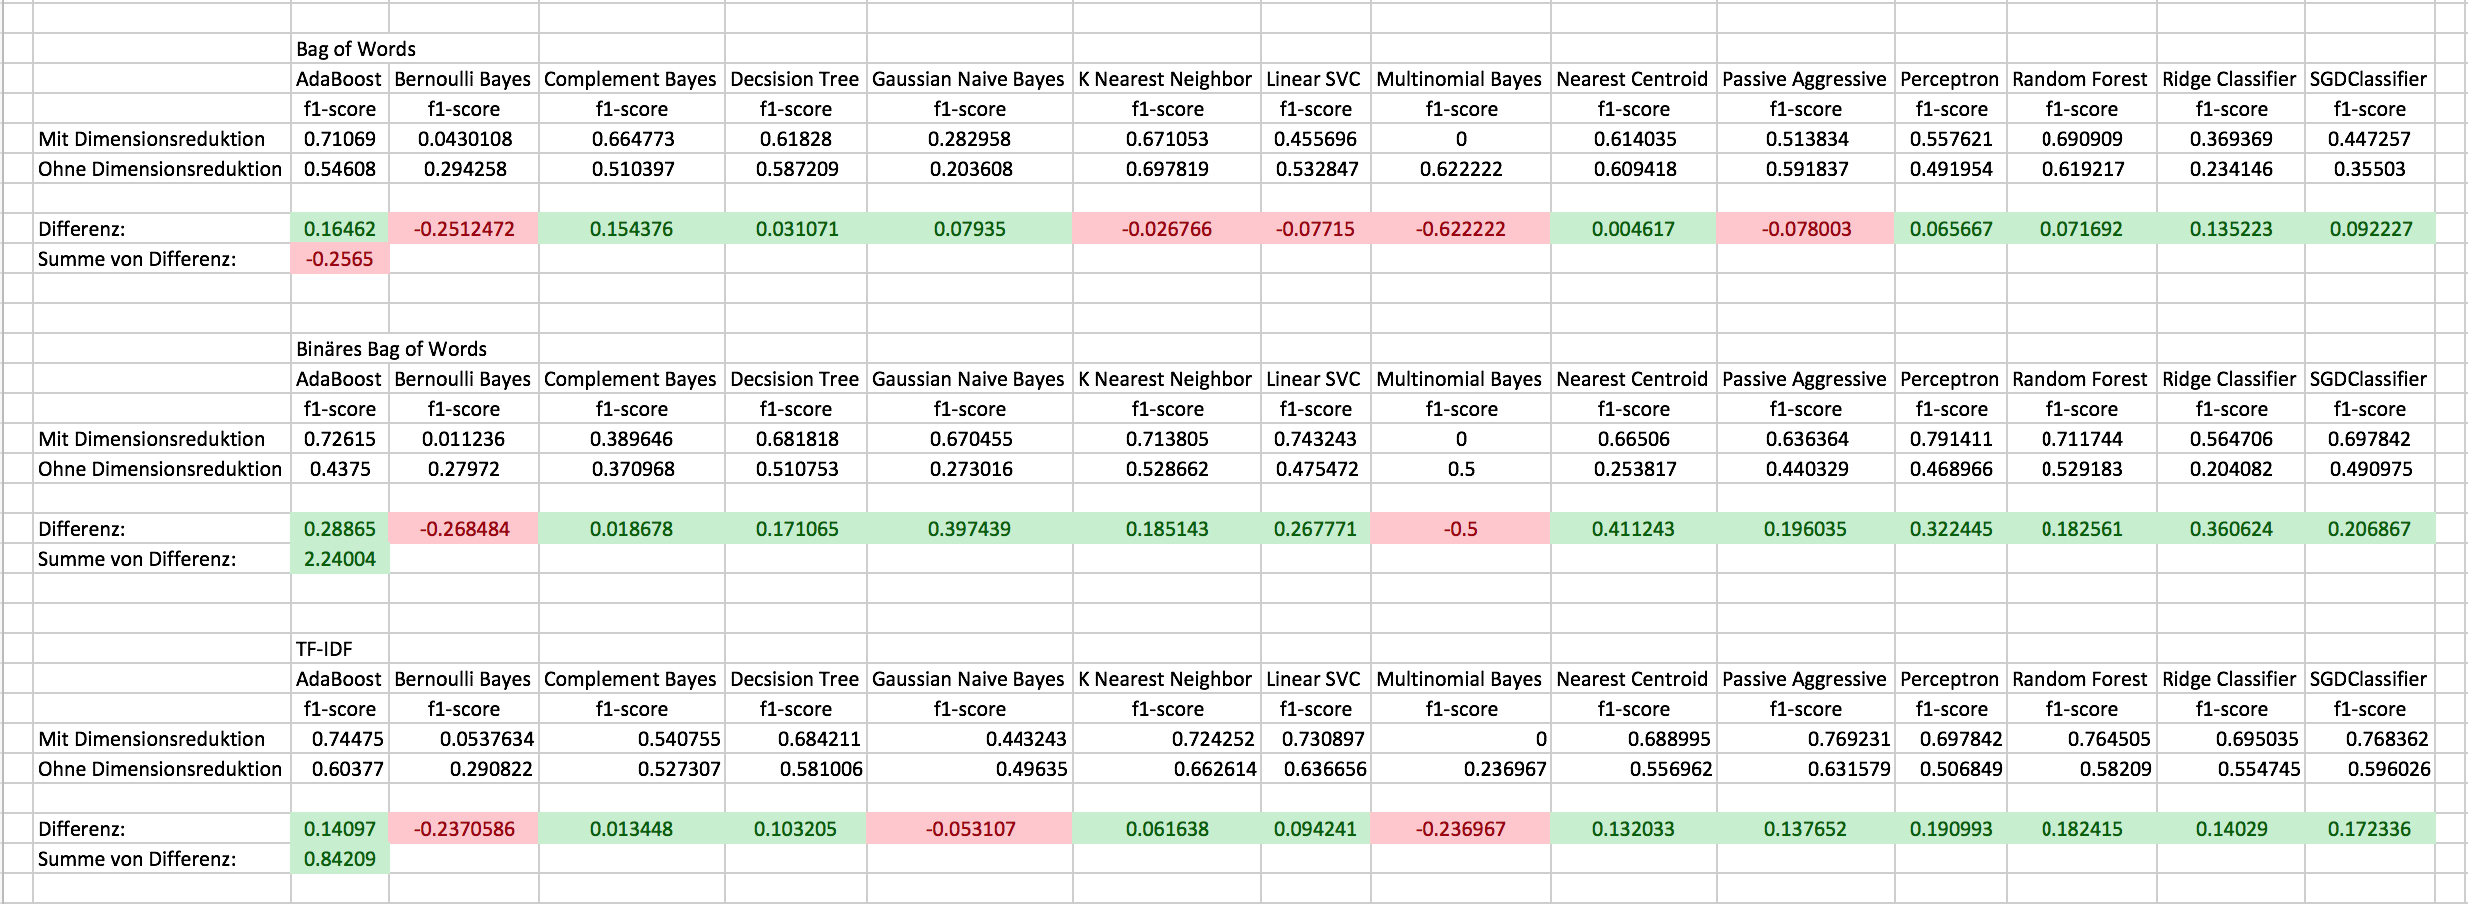
\includegraphics[width=1\columnwidth,keepaspectratio]{img/dimred.png}} 
	\caption{Grafik der Auswertung für die Dimensionsreduktion mittels LSA}
	\label{abb:dimred}
\end{figure}
\subsection{Angabe von Klassenverteilung}
\subsubsection{Beschreibung der Komponente}
\subsubsection{Methoden}
Da die Daten aus dem Goldstandard eine sehr ungleiche Verteilung von positiven und negativen Samples aufweist, wurde die Klassengewichtung anhand dieser Verteilung berechnet.
Die Gewichtung, auf ein positives Sample folgen 10.32 negative Samples, wurde den Algorithmen fürs Trainieren mitgegeben.
Mittels der Klassenverteilung können die Algorithmen die unterrepräsentierten Klassen, in unserem Falle die positive Klasse, stärker gewichten und den Fokus darauf setzen.
Einerseits wurden die Algorithmen ohne Klassengewichtung trainiert und validiert und andererseits mit der Angabe der Klassengewichtung.
Zu erwähnen ist, dass die Gewichtung nicht allen Algorithmen zugewiesen werden konnte, da manche Algorithmen während dem Training solche Informationen nicht verwerten können.
\subsubsection{Resultate}
Die Angabe der Klassenverteilung konnte nicht bei allen Algorithmen als Parameter angegeben werden.
Somit werden alle Bayes-Algorithmen, KNearestNeighbor und Nearest-Centroid in der Abbildung \cref{abb:classweight} nicht beachtet, da es dort zu keiner Veränderung der Scores kommt.\\
Bei beiden \glqq Bag of Words\grqq{} Methoden erzielt die Angabe der Klassenverteilung eine durchschnittliche Verbesserung der F1-Scores.
Einzelne Algorithmen reagieren negativ auf die Angabe, aber die positiven Auswirkungen übertreffen die negativen Auswirkungen.
Somit wird bei beiden \glqq Bag of Words\grqq{} Methoden die Angabe der Klassenverteilung miteinbezogen.\\
Bei der TF-IDF-Methode werden drei Algorithmen negativ und vier Algorithmen positiv beeinflusst.
Lediglich beim PassiveAgressiveClassifier gibt es eine markante Verschlechterung des F1-Scores.
Bei den anderen Algorithmen halten sich die negativen Auswirkungen im Rahmen.
Den F1-Score des PassiveAgressiveClassifier ausgenommen, sind die positiven Auswirkungen grösser als die negativen Auswirkungen.
Somit wird für TF-IDF ebenfalls die Angabe der Klassenverteilung für die nächsten Schritte beibehalten.
\begin{figure}[H]	
	\setlength{\fboxsep}{0.3pt} 
	\setlength{\fboxrule}{0.3pt} 
	\fbox{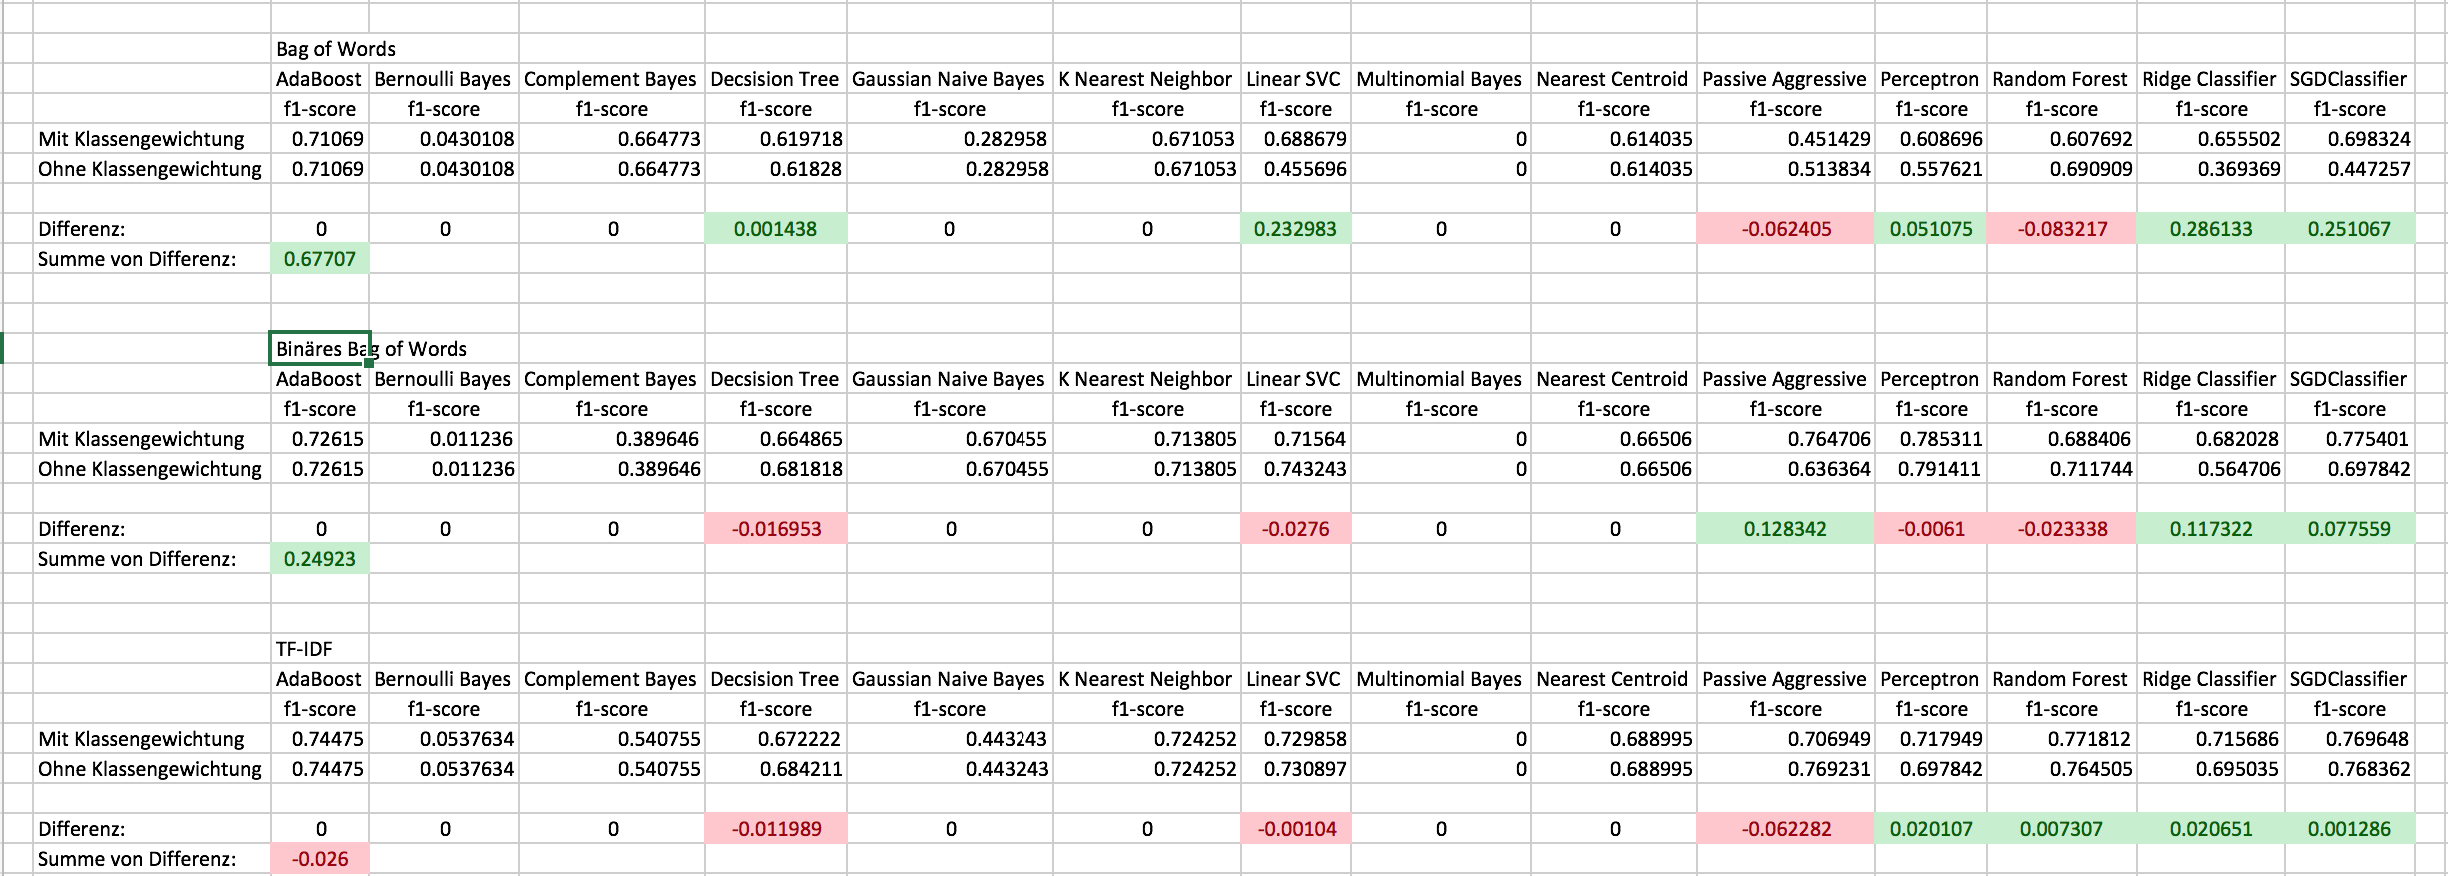
\includegraphics[width=1\columnwidth,keepaspectratio]{img/classweight.png}} 
	\caption{Grafik der Auswertung für die Klassenverteilung}
	\label{abb:classweight}
\end{figure}
\subsection{Anwendung von N-Gramme}
\subsubsection{Beschreibung der Komponente}
\subsubsection{Methoden}
Die verwendeten Feature-Extraction Methoden bieten die Möglichkeit N-Gramme als Features zu extrahieren.
Aufgrund von verschiedenen Visualisierungen der Textdaten wurde erkannt, dass es Sinn macht, die Verwendung von Bi- und Trigrammen zu prüfen.
Die Scikit-Learn Feature-Extraction Methoden bieten einfache Schnittstellen für die Extrahierung von N-Grammen.
Die Validierung von Uni-, Bi- und Trigrammen wurde für alle drei Feature-Extraction Methoden durchgeführt, die 14 Algorithmen mit den neuen Features trainiert und wieder validiert.
\subsubsection{Resultate}
Sowohl \glqq Bag of Words\grqq{} als auch TF-IDF bieten in ihrer Scikit-Learn Implementierung die Möglichkeit N-Gramme zu verwenden.
Für dieses Experiment wurden Unigramme, Bigramme und Trigramme ausgetestet.\\
Die Ergebnisse sind in der Abbildung \cref{abb:ngram} ersichtlich.
Bei beiden \glqq Bag of Words\grqq{} Methoden erzielt die Verwendung von Unigrammen die besten Ergebnisse.
Bi- und Trigramme können bei einzelnen Algorithmen ebenfalls eine Verbesserunge verzeichnen, aber im Vergleich zu Unigrammen fallen diese flächendeckend kleiner aus.
Somit werden bei beiden \glqq Bag of Words\grqq{} Varianten nur Unigramme verwendet.
Ebenfalls benötigt die Extrahierung der Features bei Bi- und Trigrammen etwa doppelt so lange, was eine enorme Performanceeinbusse ist.\\
Bei der TF-IDF-Methode erzielen Bi- und Trigramme die exakt gleichen Werte.
Dies ist zu erklären, dass die TF-IDF Methode keine relevanten Trigramme gefunden hat und somit auf Bigramme zurückgegriffen hat.
Unigramme erzielen im Durchschnitt leicht bessere Werte im Vergleich zu Bi- und Trigrammen.
Jedoch sind von den fünf besten Ergebnissen drei mit Bi-, beziehungsweise Trigrammen erzielt worden, was anhand der gelb markierten Zellen ersichtlich ist.
Da die Entscheidung bei der TF-IDF Methode nicht eindeutig gefällt werden konnte, entschieden sich die Autoren für die Anwendung von Bigrammen.
\begin{figure}[H]	
	\setlength{\fboxsep}{0.3pt} 
	\setlength{\fboxrule}{0.3pt} 
	\fbox{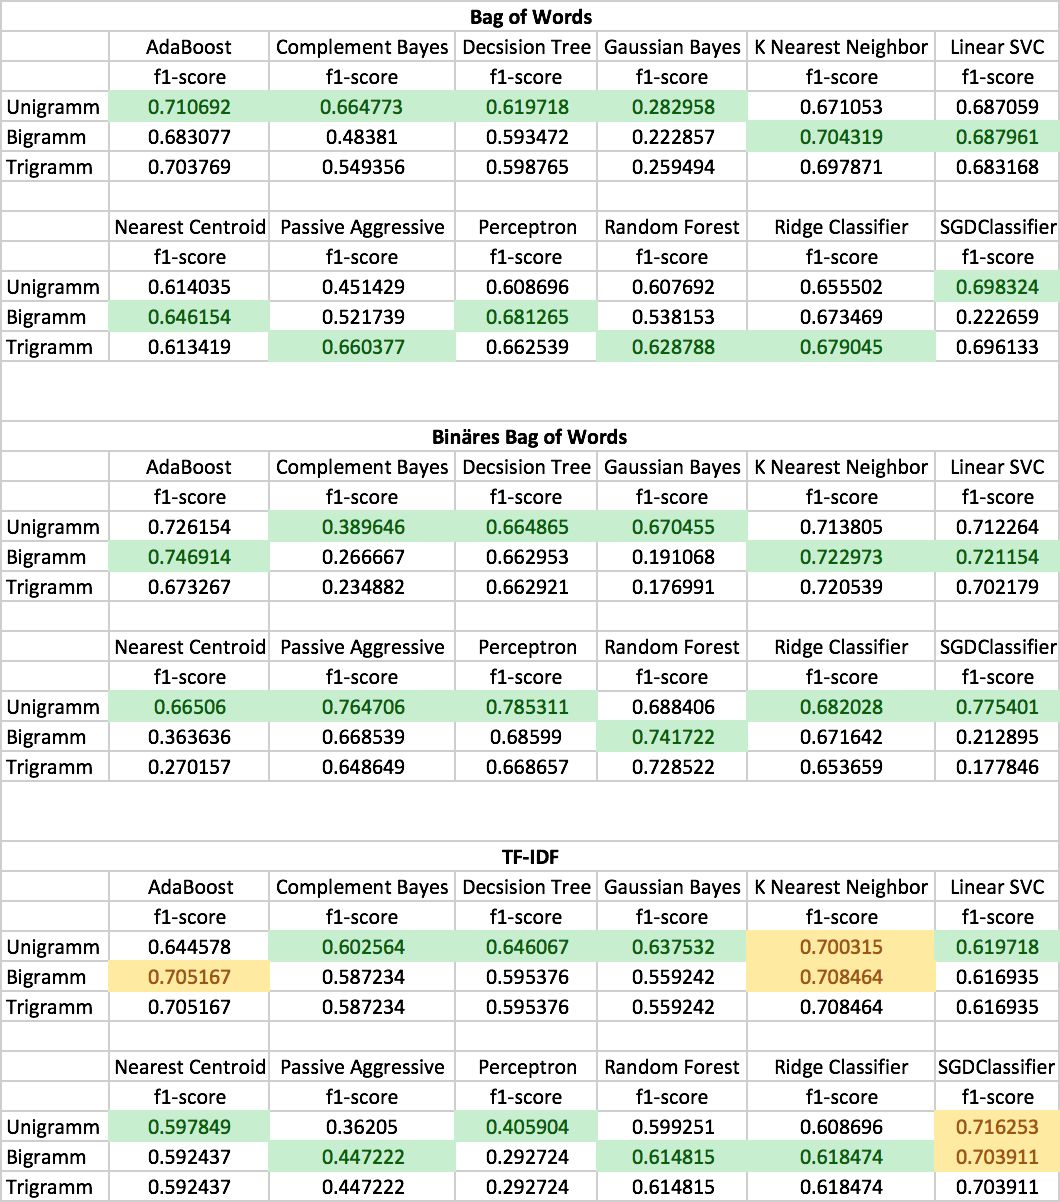
\includegraphics[width=1\columnwidth,keepaspectratio]{img/ngram.png}} 
	\caption{Grafik der N-Gramme Auswertung}
	\label{abb:ngram}
\end{figure}
\subsection{Anwendung von fortgeschrittenen Preprocessingschritten}
\subsubsection{Beschreibung der Komponente}
\subsubsection{Methoden}
Fortschrittliche Preprocessingschritte haben die Aufgabe den Text weiter zu modifizieren und die Extrahierung von zusätzlichen Informationen zu vereinfachen.
Im Kontext vom Machine-Learning Teil zählen folgende Preprocessingschritte zu den fortschrittlichen Funktionen:
\begin{itemize}
	\item Das Markieren von Preisen mit entsprechenden Tags
	\item Die Stammformreduktion
	\item Das Entfernen von Stopwörtern
	\item Das Markieren von Information, die sich auf Getränke beziehen
\end{itemize}
Diese fortschrittlichen Funktionen können ebenfalls im Unterkapitel \ref{preprocessing} nachgelesen werden.
Es wurden die Auswirkungen von jeglichen Kombinationen der fortgeschrittenen Preprocessingschritten getestet.
Bei vier verschiedenen Arten ergeben sich 16 verschiedene Kombinationen.
\subsubsection{Resultate}
Das fortschrittliche Preprocessing erzielt bei allen drei Feature-Extraction Methoden keine eindeutigen Resultate.\\
Bei der \glqq Bag of Words\grqq{} Methode erreicht die Konfiguration \glqq config8\grqq{} mit dem Preisdetektor, der Stoppwörterentfernung und der Stammformreduktion die grössten positiven Einwirkungen.
Sieben Algorithmen können mit dieser Konfiguration ihre F1-Scores verbessern.
Somit wird für \glqq Bag of Words\grqq{} die Konfiguration \glqq config8\grqq{} weiter benutzt.\\
Bei der binären \glqq Bag of Words\grqq{} Methode gibt es bei keiner Konfiguration irgendwelche flächendeckenden Verbesserungen.
Es gibt jeweils nur vereinzelte Algorithmen, welche ihre Scores verbessern können.
Da keine Konfiguration eindeutig als Verbesserung angesehen werden kann, wird bei dieser Variante keine fortschrittlichen Preprocessingschritte angewendet.\\
Bei der TF-IDF-Methode gibt es ebenfalls keine eindeutigen Verbesserungen bei irgendeiner Konfiguration.
Es können vereinzelte Algorithmen ihre Scores verbessern, aber es findet nie flächendeckend eine Verbesserung statt.
Bei der Konfiguration \glqq config5\grqq{} erzielt AdaBoost den höchsten Wert über alle Konfigurationen gesehen, aber die anderen Algorithmen werden nur leicht beeinflusst.
Um bei der weiteren Ermittlung von Optimierungen nicht nur auf ein Algorithmus zu setzen, wird bei TF-IDF kein fortschrittliches Preprocessing angewendet.
\\\\
Die Auswertung für das fortschrittliche Preprocessing kann im Anhang gefunden werden.
\subsection{Anzahl extrahierter Features}
\subsubsection{Beschreibung der Komponente}
\subsubsection{Methoden}
Jeder Algorithmus verhaltet sich mit der Änderung der Anzahl Features unterschiedlich.
Um eine optimale Anzahl an Features zu ermitteln, musste schrittweise die Anzahl Features erhöht werden, die Algorithmen mit der neuen Anzahl trainiert und schlussendlich validiert werden.
Dies ist ein recht rechenintensives Unterfangen, führt in der Regel jedoch zu spürbaren Verbesserungen der Scores bei allen Algorithmen, sofern ein lokales Maximum der jeweiligen Algorithmen gefunden werden kann.
Die Messungen wurden mit einer Anzahl Features von 10 gestartet und schrittweise um 25 Features erhöht, bis schlussendlich eine maximale Anzahl von 400 Features erreicht wurde.
Da die Rechenzeit stetig mit der Erhöhung von Features steigt, wurde die Grenze bei 400 Features gesetzt.
Grundsätzlich macht eine Begrenzung der Features Sinn, da ab einer gewissen Anzahl Features die Algorithmen mit der Handhabung der Features überfordert sind und dies sich dementsprechend auf schlechteren Scores widerspiegelt.
\subsubsection{Resultate}
Für alle drei Feature-Extraction Methoden wurde ein Liniendiagramm für F1-Score, Precision und Recall erstellt.
Aus diesen Grafiken kann entnommen werden, bei welcher Feature-Anzahl welcher Algorithmus den besten Score erzielt.
Für die weitere Auswertung sind die Grafiken für F1-Score und Precision massgebend und werden weiter analysiert.
\subsubsection{Bag of Words}
In der Abbildung \cref{abb:bow-f1} ist ersichtlich, dass mit \glqq Bag of Words\grqq{} der Algorithmus AdaBoost bei 100 Features mit Abstand den besten F1-Score erzielt und fast die 0.8 Marke erreicht.
Ebenfalls kann der LinearSVC Algorithmus einen guten F1-Score erzielen und teilt sich mit AdaBoost die besten Werte.
Ersichtlich ist ebenfalls, dass die meisten Algorithmen sich zwischen 0.6 und 0.7 bewegen und das vereinzelte Klassifizierer mit ihren Werten auf und ab springen.\\
Die springenden Algorithmen Perceptron, SGDClassifier und PassiveAgressiveClassifier sind alle von der Familie \glqq Linear\_Model\grqq{}. Ein Grund für das auffällige Verhalten wurde nicht gefunden.
Da der F1-Score vom Recall und der Precision abgeleitet wird, sind die Sprünge in der Abbildung \cref{abb:bow-f1} auf die ähnlichen Sprünge aus der Precision-Grafik \cref{abb:bow-pre} zurückzuführen.\\
\begin{figure}[H]	
	\setlength{\fboxsep}{0.3pt} 
	\setlength{\fboxrule}{0.3pt} 
	\fbox{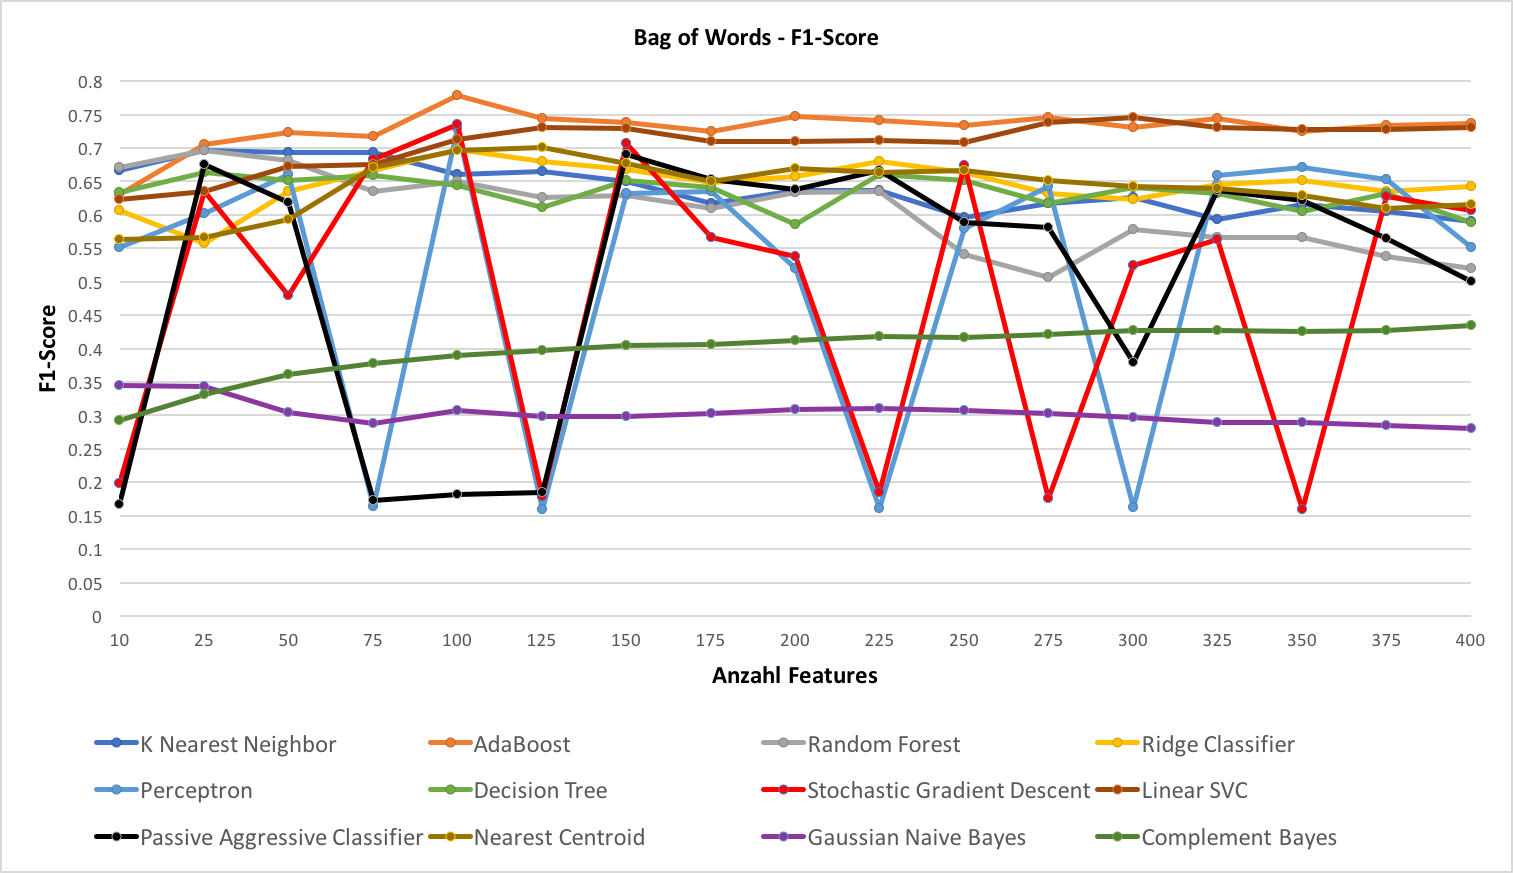
\includegraphics[width=1\columnwidth,keepaspectratio]{img/bow-f1.png}} 
	\caption{Grafik des F1-Score-Verlaufs bei Bag of Words}
	\label{abb:bow-f1}
\end{figure}
Bei der Precision, welche in der Abbildung \cref{abb:bow-pre} aufgezeigt wird, ist der RandomForest Algorithmus der mit Abstand beste Klassifizierer.
Vereinzelt erreicht RandomForest eine Precision von 1.0 und ist stetig über 0.8.\\
Die oben erwähnten Sprünge der linearen Modelle sind deutlich im Precision-Verlauf in der Abbildung \cref{abb:bow-pre} ersichtlich.
\begin{figure}[H]	
	\setlength{\fboxsep}{0.3pt} 
	\setlength{\fboxrule}{0.3pt} 
	\fbox{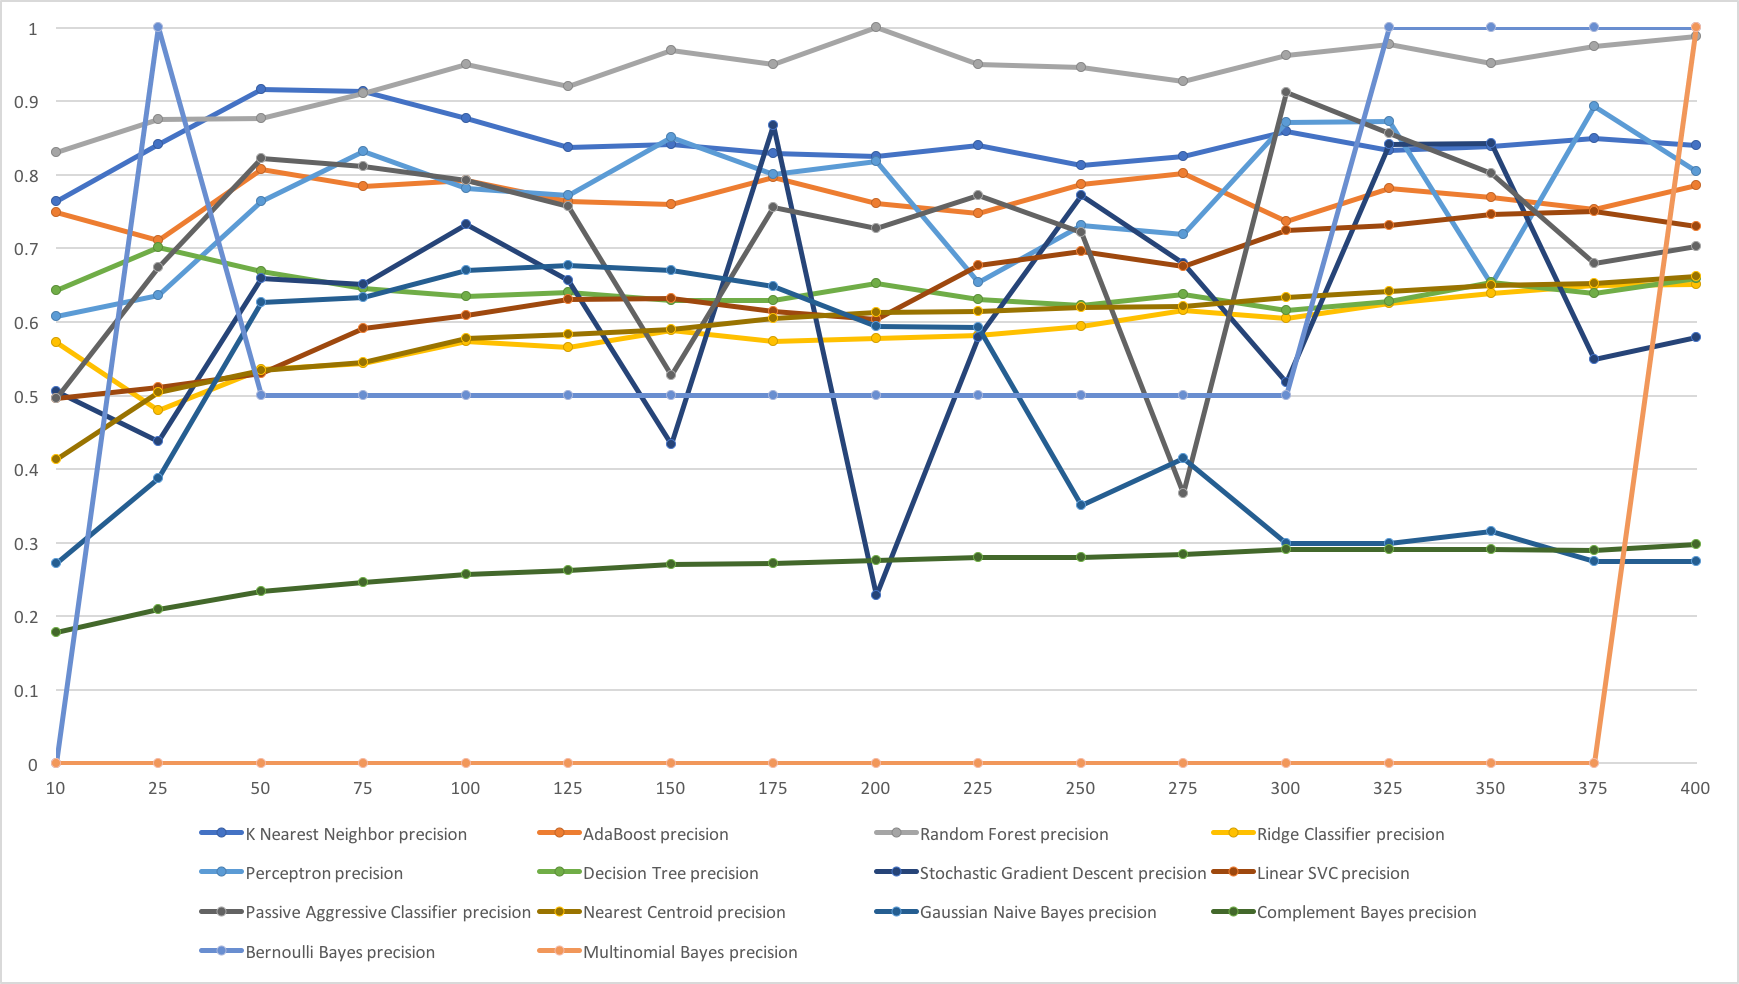
\includegraphics[width=1\columnwidth,keepaspectratio]{img/bow-pre.png}} 
	\caption{Grafik des Precision-Verlaufs bei Bag of Words}
	\label{abb:bow-pre}
\end{figure}
\subsubsection{Binäres Bag of Words}
Bei der Methode \glqq binäres Bag of Words\grqq{} können mehrere Algorithmen einen F1-Score nahe der 0.8 Grenze verbuchen.
In der Abbildung \cref{abb:bow-bin-f1} ist klar erkennbar, dass die meisten Algorithmen einen F1-Score zwischen 0.6 und 0.8 erzielen.
Der beste Algorithmus ist Perceptron, welcher mit 325 Features einen F1-Score von 0.8 verzeichnet.\\
Der SGDClassifier erreicht ebenfalls einen F1-Score von 0.8, jedoch mit einer höheren Anzahl von Features.
Dies bedeutet das SGDClasifier potenziell länger für die Feature-Extraction benötigt und somit ist Perceptron der favorisierende Algorithmus bei dieser Variante.\\
\begin{figure}[H]	
	\setlength{\fboxsep}{0.3pt} 
	\setlength{\fboxrule}{0.3pt} 
	\fbox{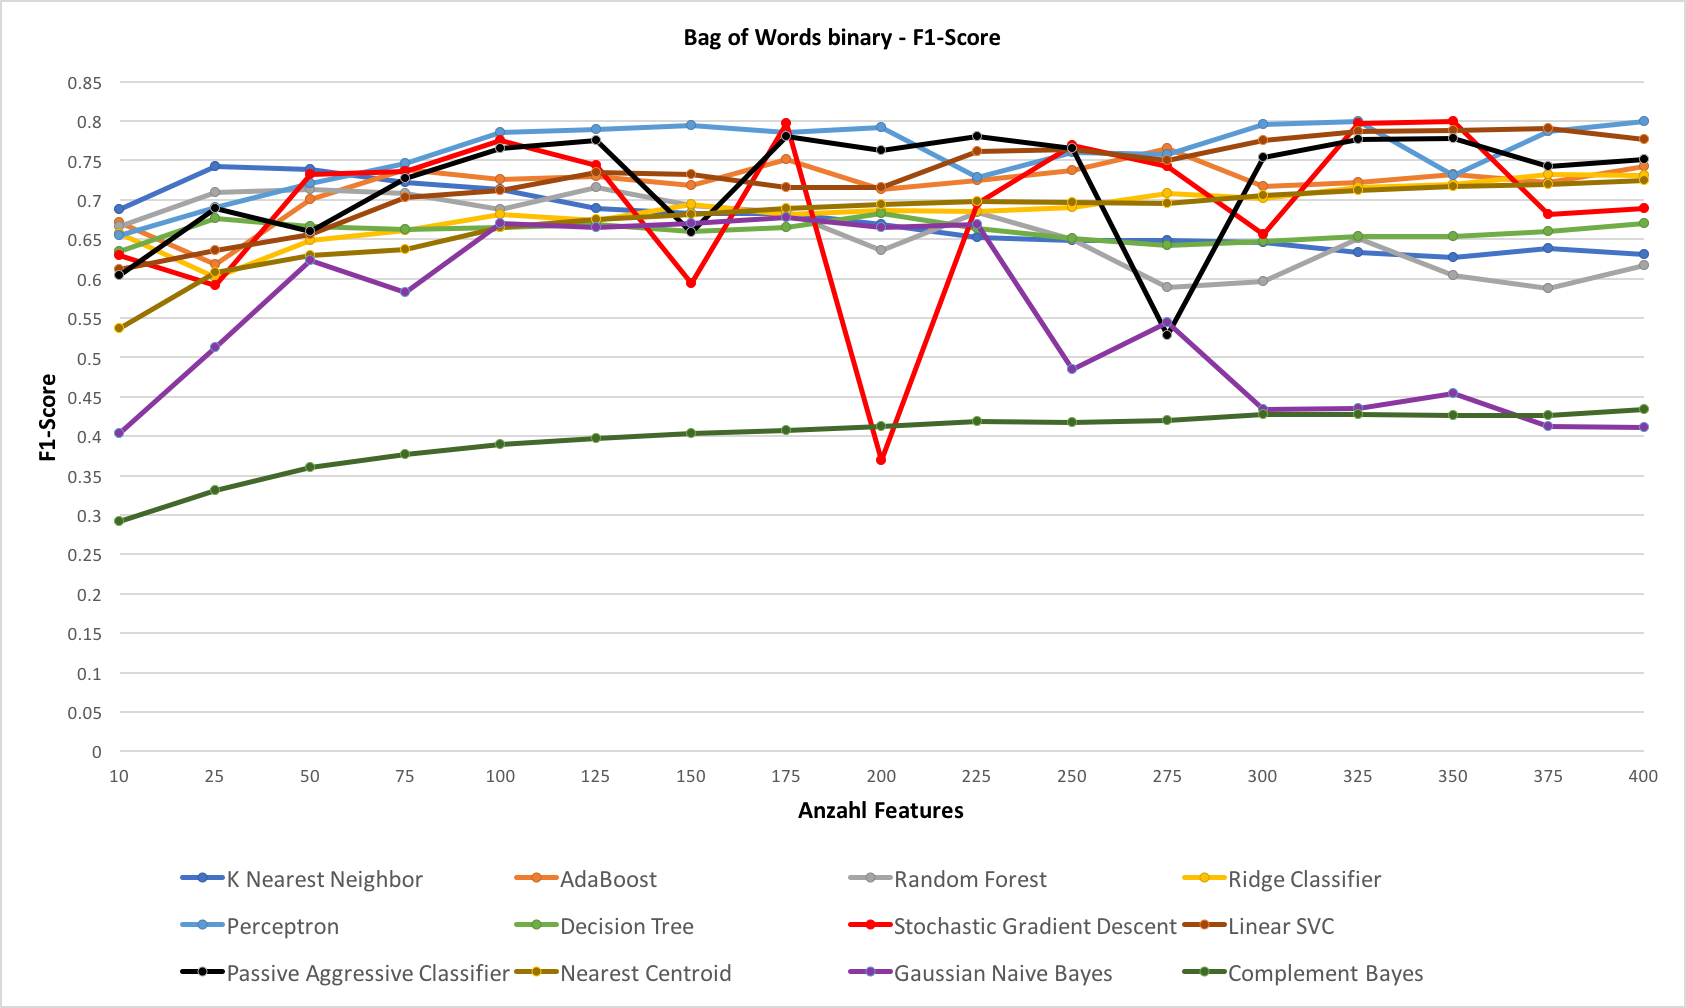
\includegraphics[width=1\columnwidth,keepaspectratio]{img/bow-bin-f1.png}} 
	\caption{Grafik des F1-Score-Verlaufs bei binärem Bag of Words}
	\label{abb:bow-bin-f1}
\end{figure}
Bei der Precision, die in der Abbildung \cref{abb:bow-bin-pre} aufgezeigt wird, ist der RandomForest Algorithmus ebenfalls die beste Wahl.
Er erreicht wieder die höchsten Prcecision-Werte bei fast jeder Anzahl an Features.\\
Die Sprünge der linearen Modelle, welche bereits bei der oberen \glqq Bag of Words\grqq{} Methode dargestellt wurden, sind ebenfalls wieder in der Precision-Grafik \cref{abb:bow-bin-pre} und der oberen F1-Score-Grafik \cref{abb:bow-bin-f1} zu erkennen.
\begin{figure}[H]	
	\setlength{\fboxsep}{0.3pt} 
	\setlength{\fboxrule}{0.3pt} 
	\fbox{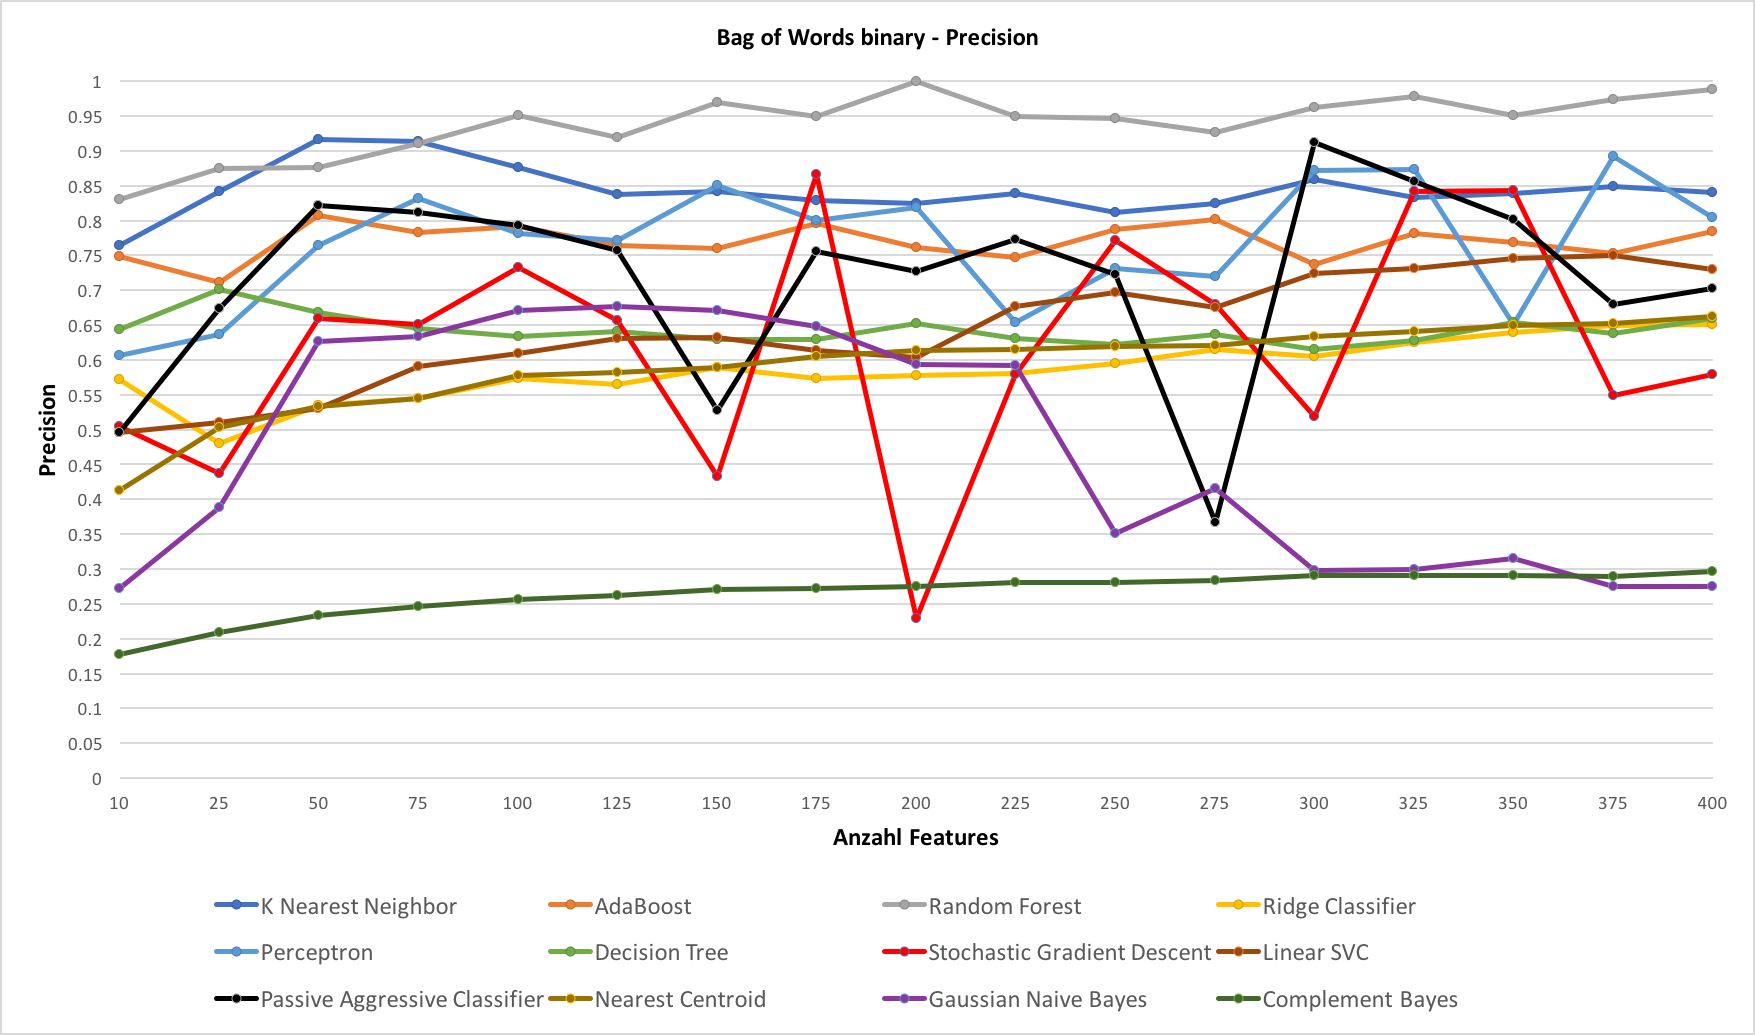
\includegraphics[width=1\columnwidth,keepaspectratio]{img/bow-bin-pre.png}} 
	\caption{Grafik des Precision-Verlaufs bei binärem Bag of Words}
	\label{abb:bow-bin-pre}
\end{figure}
\subsubsection{TF-IDF}
Bei der Verwendung von TF-IDF sind mehrere Algorithmen mit ihren F1-Scores im Bereich 0.7 bis 0.8.
In der Abbildung \cref{abb:tfidf-f1} ist erkennbar, dass der SGDClassifier Algorithmus als einziger die Grenze von 0.8 durchbrechen kann und ist somit der Algorithmus mit dem besten F1-Score.\\
Auch bei der TF-IDF Methode sind wieder Sprünge bei den linearen Modellen in beiden Grafiken \cref{abb:tfidf-f1} und \cref{abb:tfidf-pre} deutlich ersichtlich.
\begin{figure}[H]	
	\setlength{\fboxsep}{0.3pt} 
	\setlength{\fboxrule}{0.3pt} 
	\fbox{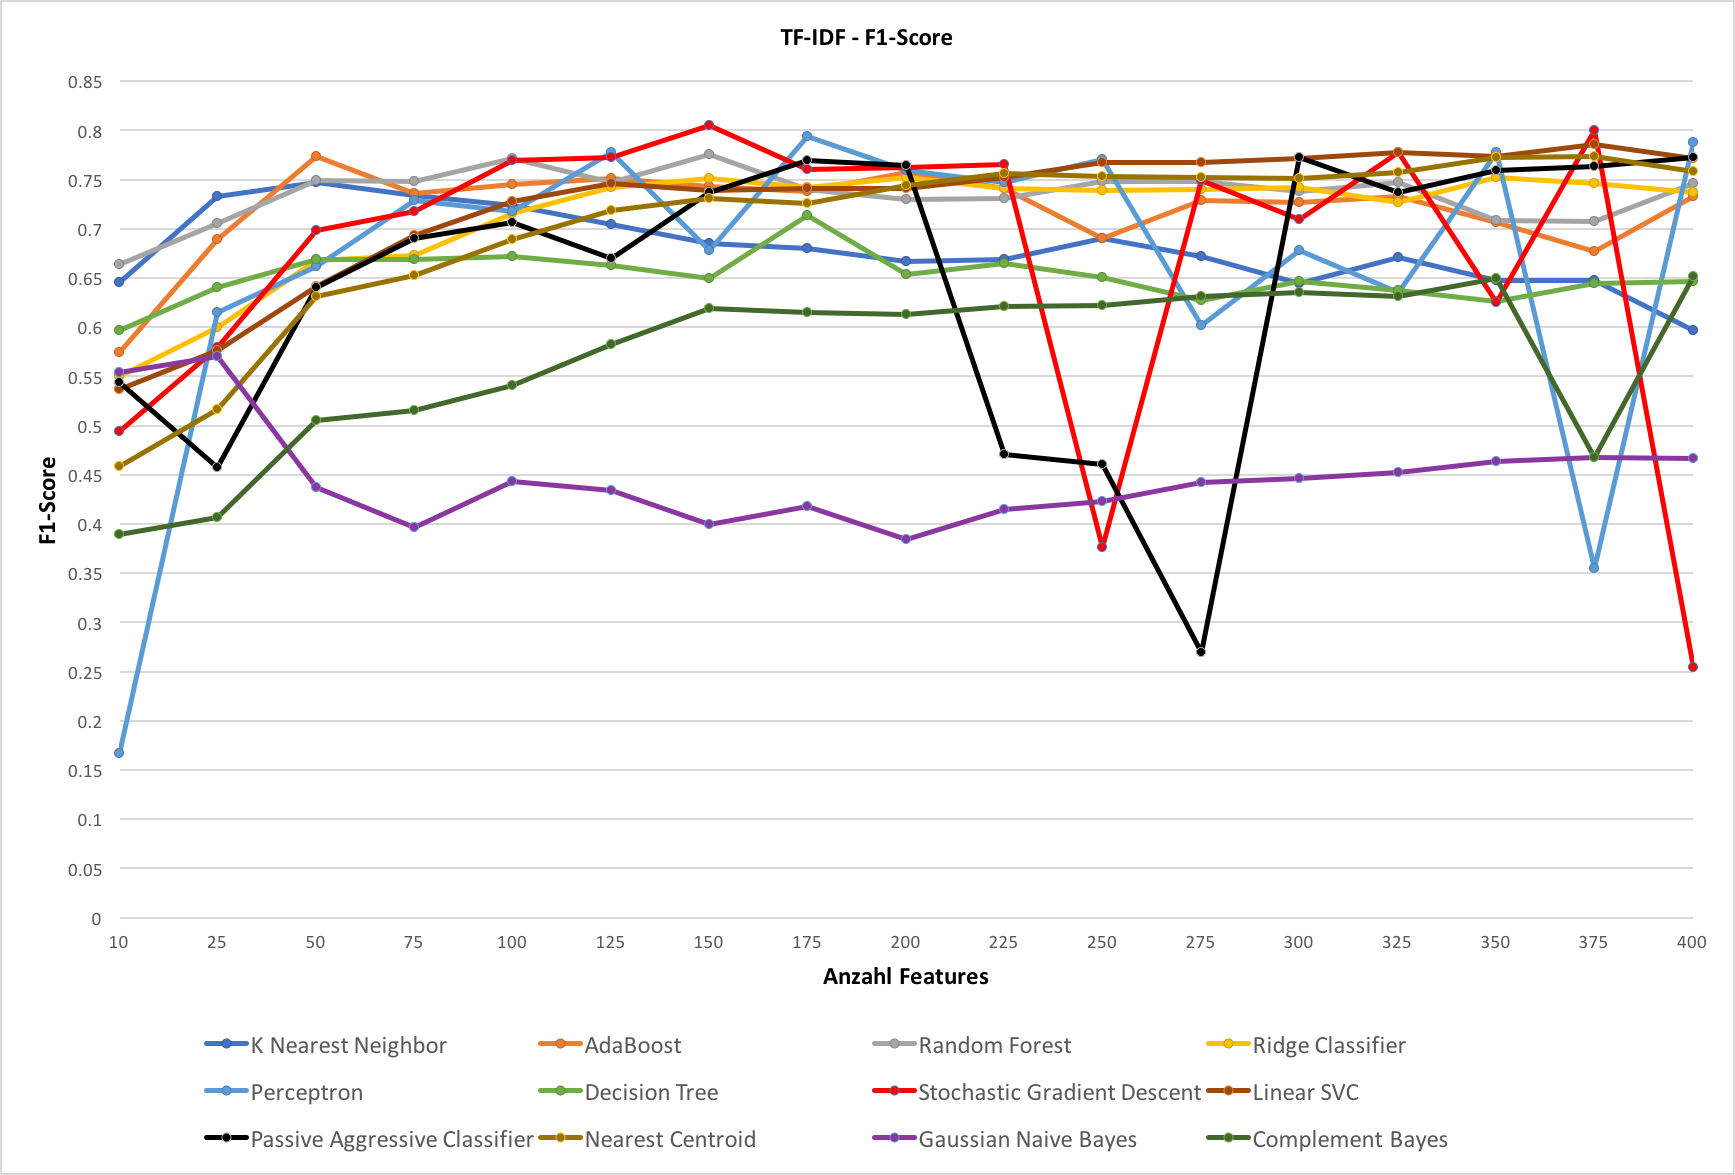
\includegraphics[width=1\columnwidth,keepaspectratio]{img/tfidf-f1.png}} 
	\caption{Grafik des F1-Score-Verlaufs bei TF-IDF}
	\label{abb:tfidf-f1}
\end{figure}
Bei der Precision ist der RandomForest Algorithmus ebenfalls wieder der Spitzenreiter.
Er erzielt bei fast jeder Anzahl von Features die beste Precision und kann bei 325 Features sein Maximum erreichen.
\begin{figure}[H]	
	\setlength{\fboxsep}{0.3pt} 
	\setlength{\fboxrule}{0.3pt} 
	\fbox{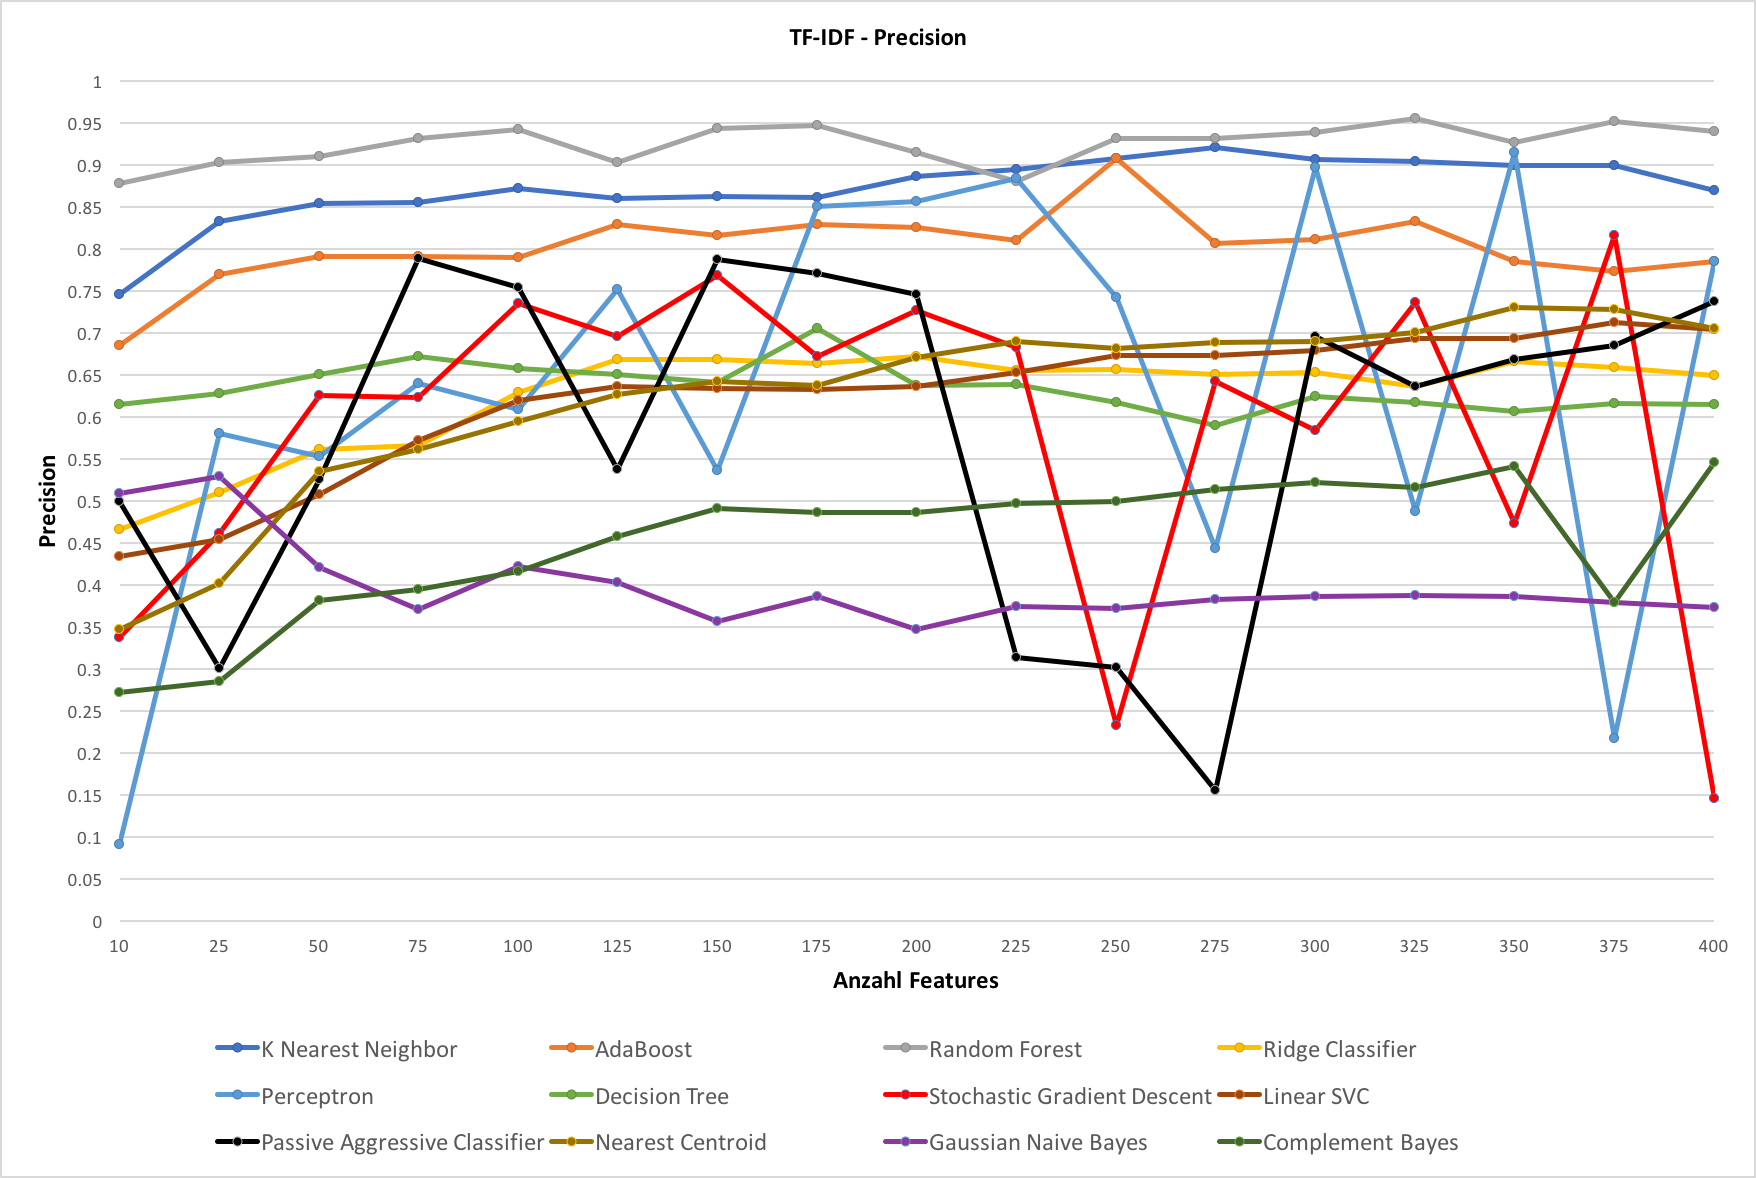
\includegraphics[width=1\columnwidth,keepaspectratio]{img/tfidf-pre.png}} 
	\caption{Grafik des Precision-Verlaufs bei TF-IDF}
	\label{abb:tfidf-pre}
\end{figure}
\subsection{Hyperparametertuning}
\subsubsection{Beschreibung der Komponente}
\subsubsection{Methoden}
Als letzter Schritt der Algorithmenoptimierung wurde eine ausführliche Hyperparametersuche mit Kreuzvalidierung durchgeführt.
Es wurde eine Kreuzvalidierung von fünf ausgewählt, um Overfitting gegenzuwirken.
Es wurden jeweils die Modelle mit den drei besten F1-Scores und den besten Precisions kreuzvalidiert.
Für jedes Modell wurde eine Liste von anpassbaren Parametern zusammengestellt.
Für jeden Parameter wurde ein Bereich von möglichen Werten angegeben.
Mittels der Funktion \glqq GridSearchCV\grqq{}\footnote{\url{https://scikit-learn.org/stable/modules/generated/sklearn.model_selection.GridSearchCV.html}abgerufen am: 07.05.2019} von Scikit-Learn wurde die Hyperparametersuche für die Optimierung des F1-Scores durchgeführt.\\
Je nach Algorithmus und Grösse der Parameterliste kann die Hyperparametersuche extrem lange dauern.
Ebenfalls ist es möglich, dass die Standardparameter bereits ein Optimum darstellen und keine besseren Parameter gefunden werden.
\subsubsection{Resultate}
Die sechs Modelle, welche aus dem vorherigen Experiment, als die besten entnommen wurden, werden mittels Kreuzvalidierung auf optimale Hyperparameter durchsucht.
\subsubsection{Modelle mit bestem F1-Score}
Die drei Modelle AdaBoost, SGDClassifier und Perceptron konnten die besten F1-Scores erzielen.\\
\begin{table}[H]
	\caption{Auwertung Hyperparametertuning für AdaBoost mit binärem Bag of Words}
	\centering
	\label{tab:ada}
	\begin{tabular}{|l|l|l|l|}
		\hline
		& F1-Score & Precision & Recall\\
		\hline
		Vor Hyperparametertuning & 0.778 & 0.837 & 0.727 \\
		Nach Hyperparametertuning & 0.788 & 0.817 & 0.761 \\
		\hline
	\end{tabular}
\end{table}
\begin{table}[H]
	\caption{Auwertung Hyperparametertuning für Perceptron mit Bag of Words}
	\centering
	\label{tab:per}
	\begin{tabular}{|l|l|l|l|}
		\hline
		& F1-Score & Precision & Recall\\
		\hline
		Vor Hyperparametertuning & 0.8 & 0.872 & 0.739 \\
		Nach Hyperparametertuning & 0.579 & 0.426 & 0.903 \\
		\hline
	\end{tabular}
\end{table}
\begin{table}[H]
	\caption{Auwertung Hyperparametertuning für SGDClassifier mit TF-IDF}
	\centering
	\label{tab:sgd}
	\begin{tabular}{|l|l|l|l|}
		\hline
		& F1-Score & Precision & Recall\\
		\hline
		Vor Hyperparametertuning & 0.805 & 0.768 & 0.847 \\
		Nach Hyperparametertuning & 0.762 & 0.682 & 0.864 \\
		\hline
	\end{tabular}
\end{table}
In der Tabelle \cref{tab:ada} ist auffällig, dass AdaBoost als einziges Modell bessere Hyperparameter mittels Hyperparemtertuning finden konnte.\\
AdaBoost kann seinen Recall verbessern und gleichzeitig verschlechtert sich seine Precision.
Da die Recallsteigerung grösser als der Precisionabfall ist, wird der F1-Score nach oben korrigiert.\\
Die anderen beiden Modelle Perceptron in Tabelle \cref{tab:per} und SGDClassifier in der Tabelle \cref{tab:sgd} erzielen mit den neuen Parametern schlechtere Werte.
Beide können den Recall verbessern, jedoch müssen sie massive Gefälle bei der Precision einbüssen.
Da die Precision viel stärker abgenommen, als der Recall zugenommen hat, wird der F1-Score schlechter.\\
Somit sind die Standardparameter für Perceptron und SGDClassifier für diesen \glqq Use-Case\grqq{} bereits optimal gewählt worden, da beim Hyperparametertuning eine ausführliche Liste von veränderbaren Parametern keine Verbesserung erzielen konnte.\\
Perceptron hat im Vergleich zum SGDClassifier einen leicht tieferen F1-Score, jedoch ist seine Precision deutlich höher.
Da für den schlussendlichen \glqq Use-Case\grqq{} Precision wichtig ist, wird das Perceptron-Modell für weitere Auswertungen verwendet.
\subsubsection{Modelle mit bester Precision}
Das Modell RandomForest kann für alle drei Feature-Extraction Methoden jeweils den besten Precision-Score erzielen.\\
\begin{table}[H]
	\caption{Auwertung Hyperparametertuning für RandomForest mit binärem Bag of Words}
	\centering
	\label{tab:bow-rf}
	\begin{tabular}{|l|l|l|l|}
		\hline
		& F1-Score & Precision & Recall\\
		\hline
		Vor Hyperparametertuning & 0.636 & 1.0 & 0.466 \\
		Nach Hyperparametertuning & 0.736 & 0.8 & 0.682 \\
		\hline
	\end{tabular}
\end{table}
\begin{table}[H]
	\caption{Auwertung Hyperparametertuning für RandomForest mit Bag of Words}
	\centering
	\begin{tabular}{|l|l|l|l|}
		\hline
		& F1-Score & Precision & Recall\\
		\hline
		Vor Hyperparametertuning & 0.636 & 1.0 & 0.466 \\
		Nach Hyperparametertuning & 0.768 & 0.829 & 0.716 \\
		\hline
	\end{tabular}
\end{table}
\begin{table}[H]
	\caption{Auwertung Hyperparametertuning für RandomForest mit TF-IDF}
	\centering
	\begin{tabular}{|l|l|l|l|}
		\hline
		& F1-Score & Precision & Recall\\
		\hline
		Vor Hyperparametertuning & 0.747 & 0.956 & 0.614 \\
		Nach Hyperparametertuning & 0.794 & 0.823 & 0.767 \\
		\hline
	\end{tabular}
\end{table}
Alle drei Varianten können ihren F1-Score verbessern.
Die Verbesserung erfolgt nur im Bereich Recall, welcher initial bei allen drei Modellen relativ tief war.
Zusätzlich sinken bei allen drei Modellen die Precision-Scores.
Bei beiden Varianten mit Bag of Words, waren alle drei initialen Scores identisch und die Precision maximal.\\
Da in diesem Unterkapitel auf die beste Precision geachtet wird, ist das Modell aus der Tabelle \cref{tab:bow-rf} mit binärem Bag of Words und mit den Standardparametern die beste Wahl und wird für weitere Auswertungen verwendet.
\subsection{Diskussion der Experimente mittels Machine-Learning}
\section{Diskussion}
\section{Beantwortung der Forschungsfrage}
\section{Verwendete Technologien}